\documentclass[t]{beamer}
\usepackage[utf8]{inputenc}
\usetheme{Madrid}
\usepackage{lmodern}
\usepackage{amsmath,amsfonts,amssymb}
\usepackage{graphicx,xcolor,enumitem}
\setbeamertemplate{bibliography item}{\insertbiblabel}
\setitemize{label=\usebeamerfont*{itemize item}%
  \usebeamercolor[fg]{itemize item}
  \usebeamertemplate{itemize item}}

\newcommand{\ToDo}[1]{\textcolor{red}{[#1]}}

% Statistical notation:
\newcommand{\noise}{\eta}	% Noise (single component/variable)
\newcommand{\noiseSD}{\sigma}	% Standard deviation
\DeclareMathOperator{\E}{E}	% Expected value
\DeclareMathOperator{\Var}{Var}	% Variance
\renewcommand{\Re}{\operatorname{Re}}	% Real part
\renewcommand{\Im}{\operatorname{Im}}	% Imaginary part

% Discrete notation:
\newcommand{\gVec}{\mathbf{g}}	% Vector
\newcommand{\gnoise}{\widetilde{g}}	% Component
\newcommand{\gnoiseVec}{\widetilde{\mathbf{g}}}	% Vector
\newcommand{\kVec}{\mathbf{k}}	% Vector
\newcommand{\kMat}{K}	% Matrix K
\newcommand{\fVec}{\mathbf{f}}	% Vector
\newcommand{\tVec}{\mathbf{t}}	% Vector
\newcommand{\dVec}{\mathbf{d}}	% Differential operator vector
\newcommand{\trans}{\mathrm{T}}	% Matrix transpose
\newcommand{\ctrans}{*}	% Conjugate transpose
\DeclareMathOperator{\diag}{diag}	% Diagonal matrix
\DeclareMathOperator{\rank}{rank}	% Rank of a matrix
\newcommand{\noiseVec}{\mathbf{\noise}}	% Noise vector
\newcommand{\singular}{s}	% Singular values
\DeclareMathOperator{\trace}{trace}		% Trace
\newcommand{\dct}[1]{\breve{#1}}	% DCT of vector

% Regularization notation:
\newcommand{\regparam}{\alpha}
\newcommand{\R}{R_{\regparam}}	% Regularization matrix
\newcommand{\regf}{\fVec_{\regparam}}	% Regularized solution
\DeclareMathOperator*{\argmax}{arg\,max}
\DeclareMathOperator*{\argmin}{arg\,min}
\newcommand{\filt}{\phi}
\newcommand{\mfilt}{\psi}

% UPRE derivation notation:
\newcommand{\PE}{\mathbf{p}_{\regparam}}	% Predictive error
\newcommand{\regres}{\mathbf{r}_{\regparam}}	% Regularized residual
\newcommand{\A}{A_{\regparam}}	% Influence matrix
\newcommand{\U}{U}	% UPRE function

% GCV derivation notation:
\newcommand{\GCV}{G}	% GCV function

% Discrepancy principle derivation notation:
\newcommand{\D}{D}	% Discrepancy principle function

\author{Michael Byrne}
\title[Regularization Parameter Estimation]{Resolution analyses and estimation of regularization parameters for the inversion of integral equations}
\subtitle{Prospectus for Applied Mathematics PhD}
%\setbeamercovered{transparent} 
%\setbeamertemplate{navigation symbols}{} 
%\logo{} 
\institute{Arizona State University} 
\date{December 3, 2019} 
%\subject{} 

\AtBeginSection[]
{
    \begin{frame}
        \frametitle{Table of Contents}
        \tableofcontents[currentsection]
    \end{frame}
}

\begin{document}

% Title page:
\begin{frame}
\titlepage
\end{frame}

% Table of contents:
\begin{frame}
\tableofcontents
\end{frame}

\section{Introduction}

\begin{frame}
\frametitle{Inverse problems}
\begin{itemize}
\item Inverse problems are concerned with determining model parameters/characteristics from observed data
\item Historical example is the detection of Neptune (1821-1846; see \cite{Airy1847})
\item Modern examples include to deconvolution, tomography, and subsurface mapping from gravitational measurements \cite{ABT}
\end{itemize}
\begin{block}{Fredholm equation of the first kind}
Given functions $k(x,t)$ and $g(x)$, the Fredholm equation of the first kind is
\[g(x) = \int_a^b k(x,t)f(t)~dt,\]
where the function $f(t)$ is unknown. The function $k$ is called the kernel of the integral equation.
\end{block}
\end{frame}

\begin{frame}
\frametitle{Convolution of functions}
When the kernel has the form $k(x,t) = k(x-t)$ and the limits of integration are infinite, the integral equation represents the convolution of $k$ and $f$:
\[(k * f)(x) := g(x) = \int_{-\infty}^{\infty} k(x-t)f(t)~dt.\]
\begin{itemize}
\item Convolution is a ``smoothing" operation: if $k$ has compact support and $f$ is locally integrable, then $g$ exists and is continuous \cite{DebnathMikusinski2005} 
\item A truncated Gaussian function is a common kernel
\[k(x-t) = \exp\left(-w(x-t)^2\right)\]
\[k(x-t,y-s) = \exp\left(-w\left[(x-t)^2+(y-s)^2\right]\right)\]
\end{itemize}
\end{frame}

\begin{frame}
\frametitle{Convolution of functions}
As $w$ increases, the spread of the Gaussian kernel decreases: \vspace*{0.25 in}
\begin{center}
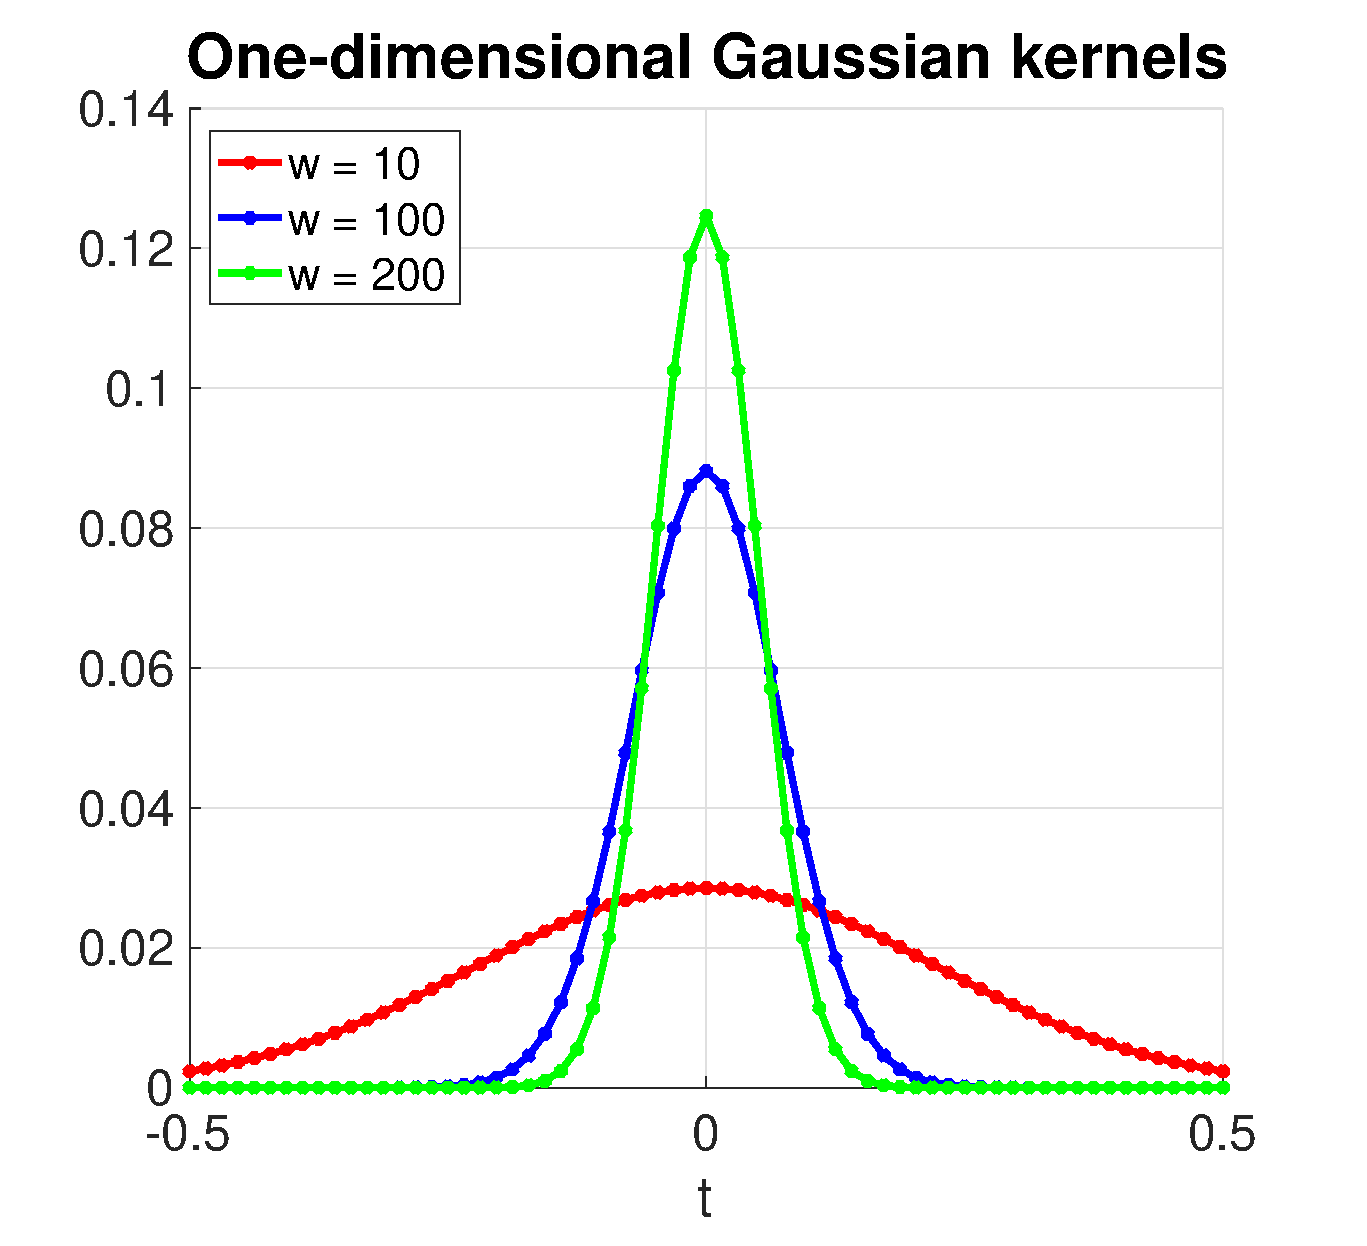
\includegraphics[width=0.45\textwidth]{Figures/GaussianKernels1D.eps}
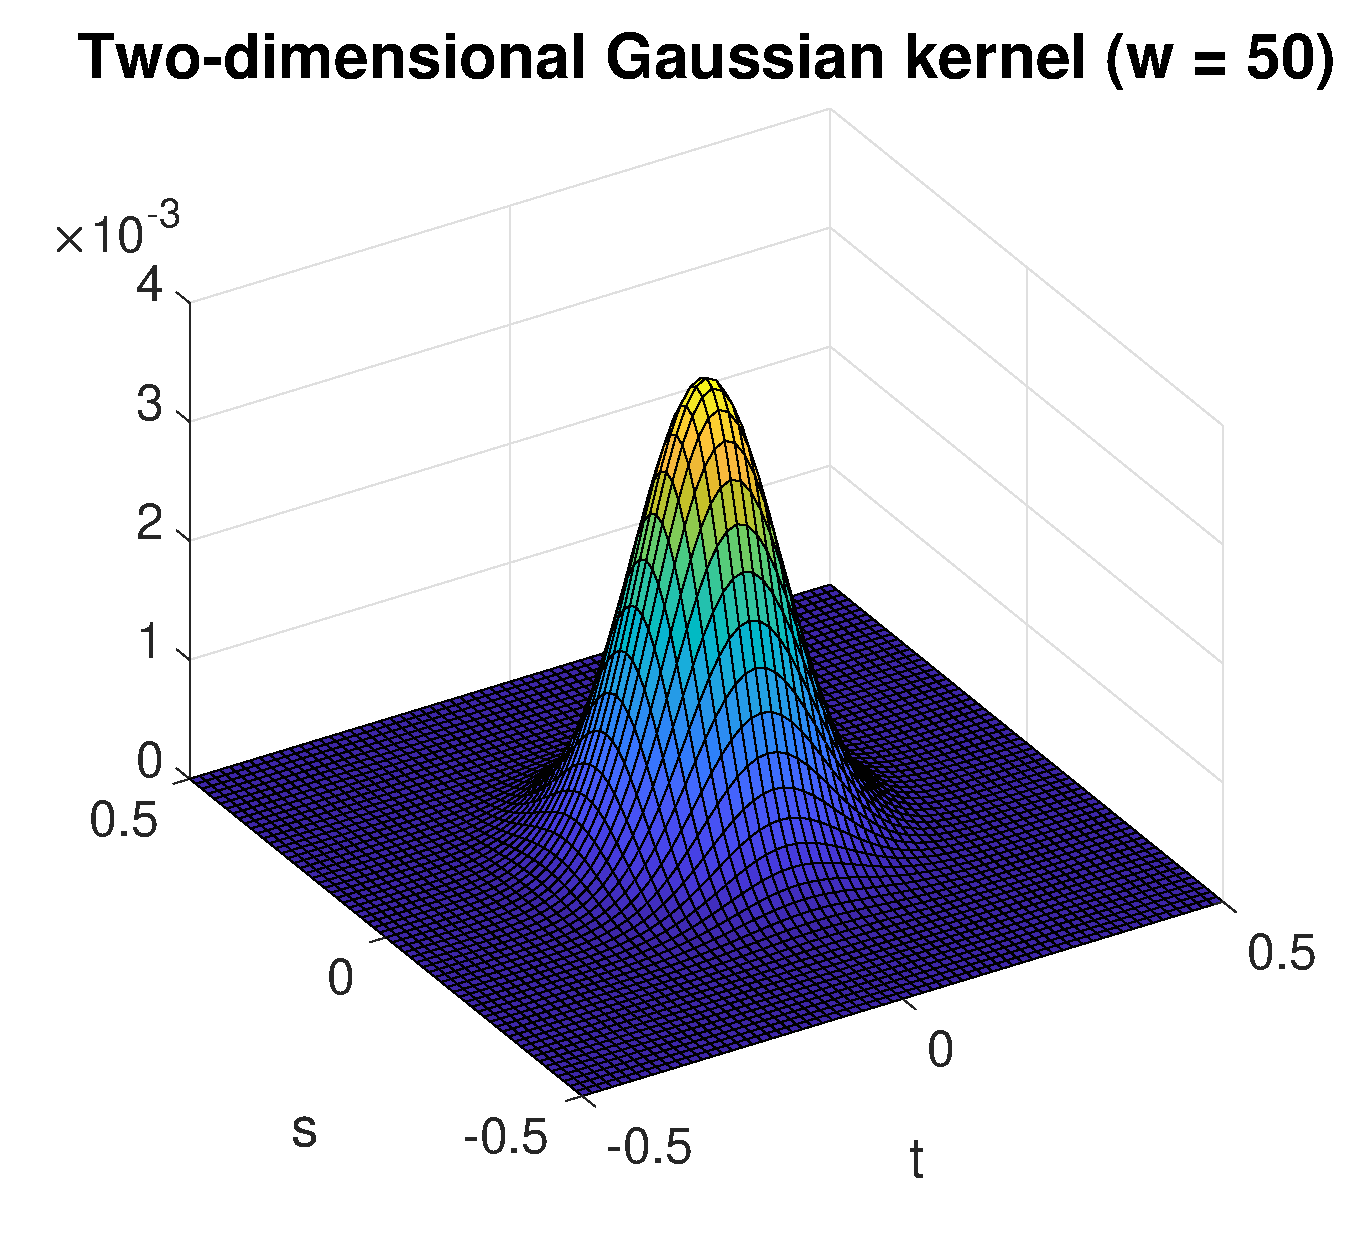
\includegraphics[width=0.45\textwidth]{Figures/GaussianKernel2D.eps}
\end{center}
\end{frame}

\begin{frame}
\frametitle{Continuous to discrete setting}
In many applications, data are finite (i.e. samples of functions)
\[\gVec = \begin{bmatrix}
g_0 \\
\vdots \\
g_{n-1}
\end{bmatrix}, \quad g_j = \sum_{\ell=-\infty}^{\infty} k_{j-\ell}f_{\ell}\]
\[(\ldots,f_{-m+1},\ldots,f_0,f_1,\ldots,f_{n-1},f_n,\ldots,f_{n+m},\ldots)\]
\[(\ldots,0,0,k_{-m+1},k_{-m+2},\ldots,k_0,\ldots,k_{m-2},k_{m-1},0,0,\ldots)\]
\begin{itemize}
\item When the kernel sequence has finitely many nonzero terms, the discrete convolution exists
\item For a quadrature method, the weights can be absorbed into the kernel sequence
\end{itemize}
\end{frame}

\begin{frame}
\frametitle{Continuous to discrete setting}
Assuming the kernel $k(x-t)$ has compact support and data $\gVec$ about $g(x)$ are finite, the resulting discrete system is finite and $\gVec$ can be expressed as the following matrix product:
\[\resizebox{.9 \textwidth}{!}{$
\begin{bmatrix}
k_{m-1} & \cdots & k_0 & \cdots & k_{-m+1} & & & & & \\
 & k_{m-1} & & k_0 & & k_{-m+1} & & & 0 & \\
 & & \ddots & \ddots & \ddots & \ddots & \ddots & & & \\
 & & & \ddots & \ddots & \ddots & \ddots & \ddots & & \\
 & 0 & & & k_{m-1} & & k_0 & & k_{-m+1} & \\
 & & & & & k_{m-1} & \cdots & k_0 & \cdots & k_{-m+1}
\end{bmatrix}\begin{bmatrix}
f_{-m} \\
\vdots \\
f_{-1} \\
f_0 \\
\vdots \\
f_{n-1} \\
f_n \\
\vdots \\
f_{n+m-1}
\end{bmatrix}$}\]
However, this system is underdetermined without imposing some boundary conditions on $f$.
\end{frame}

\begin{frame}
\frametitle{Continuous to discrete setting (1D)}
The discrete system can be rewritten as
\[\gVec = T_{l}\fVec_{l} + T\fVec + T_{r}\fVec_{r}\]
where matrices/vectors come from the following partition \cite{NeumannDCT}:
\[\resizebox{1 \textwidth}{!}{$
\left[\begin{array}{cc|cccccc|cc}
k_{m-1} & \cdots & k_0 & \cdots & k_{-m+1} & & & & & \\
 & k_{m-1} & & k_0 & & k_{-m+1} & & & 0 & \\
 & & \ddots & \ddots & \ddots & \ddots & \ddots & & & \\
 & & & \ddots & \ddots & \ddots & \ddots & \ddots & & \\
 & 0 & & & k_{m-1} & & k_0 & & k_{-m+1} & \\
 & & & & & k_{m-1} & \cdots & k_0 & \cdots & k_{-m+1} 
\end{array}\right]\left[\begin{array}{c}
f_{-m} \\
\vdots \\
f_{-1} \\
\hline 
f_0 \\
\vdots \\
f_{n-1} \\
\hline
f_n \\
\vdots \\
f_{n+m-1}
\end{array}\right]\begin{array}{c}
\vspace*{0.25 in} \\
\leftarrow \fVec_l \\
\vspace*{0.25 in} \\
\leftarrow \fVec \\
\vspace*{0.25 in} \\
\leftarrow \fVec_r \\
\vspace*{0.25 in} 
\end{array}$}\]
\end{frame}

\begin{frame}
\frametitle{Singular value decomposition (SVD)}
Given a system $\gnoiseVec = \kMat\fVec + \noiseVec$ where $\kMat$ is an $m \times n$ matrix, $\rank(\kMat) = r$, and $\noiseVec$ is a vector realization of noise, direct matrix inversion is impractical/impossible. A theoretical alternative is to express $\kMat$ using the (compact) SVD.
\[\kMat = U\Sigma{V^\ctrans}\]
\begin{itemize}[nosep]
\item $U$ is $m \times r$, $V^\ctrans$ is $r \times n$, and both $U$ and $V$ are column orthonormal.
\item $\Sigma = \diag(\singular_0,\ldots,\singular_{r-1})$ where $s_0 \geq \ldots \geq \singular_{r-1} > 0$ (the singular values)
\item If $\kMat$ is singular, the pseudoinverse $K^\dagger = V\Sigma^\dagger{U}^\ctrans$ with $\Sigma^\dagger = \diag\left(\frac{1}{\singular_0},\ldots,\frac{1}{\singular_{r-1}}\right)$ can be used for obtain a solution:
\[\kMat^\dagger{\gnoiseVec} = (V\Sigma^\dagger{U}^\ctrans)(\kMat\fVec + \noiseVec) = \fVec + \sum_{\ell=0}^{r-1} \frac{(U_{\cdot,\ell})^\ctrans{\noiseVec}}{\singular_{\ell}}V_{\cdot,\ell}\]
\end{itemize}
However, division by small singular values results in numerical instability.
\end{frame}

\begin{frame}
\frametitle{The discrete Picard condition}
A Picard plot is a graph showing the term $|(U_{\cdot,\ell})^\ctrans{\noiseVec}|/\singular_{\ell}$ in decreasing order with respect to the singular values $\singular_{\ell}$. The \textit{discrete Picard condition} is satisfied if the terms $|(U_{\cdot,\ell})^\ctrans{\noiseVec}|$ decay faster than the $\singular_{\ell}$ \cite{ABT, Hansen1990}.
\begin{center}
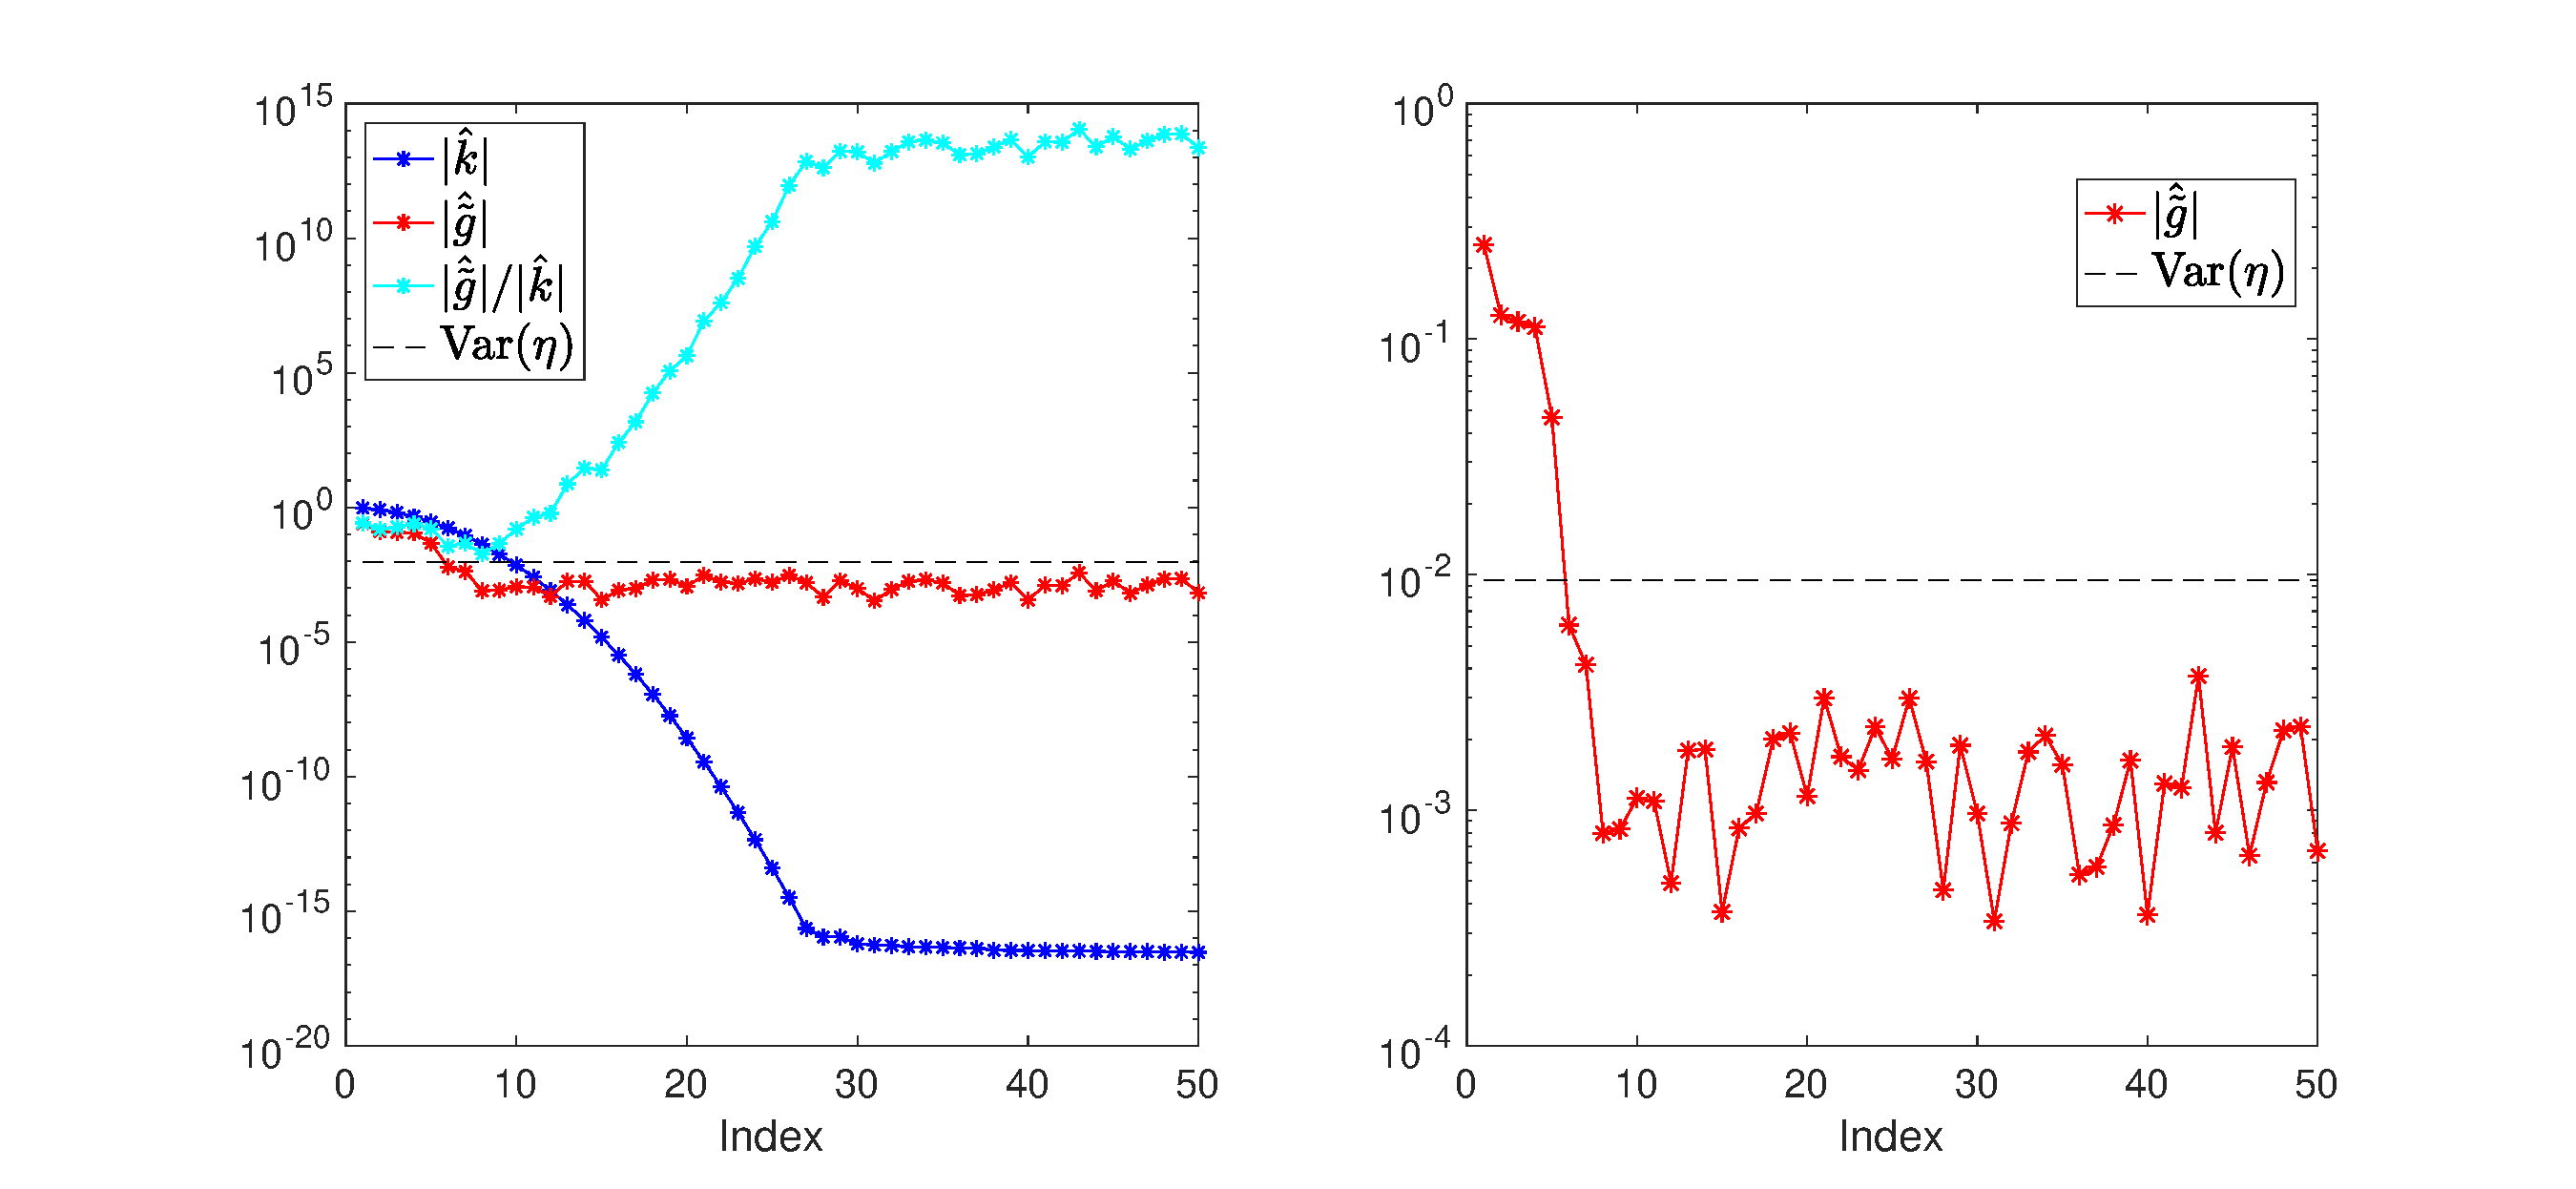
\includegraphics[scale=0.25]{Figures/PicardPlot.eps}
\end{center}
\end{frame}

\begin{frame}
\frametitle{Regularization}
\[\fVec_\regparam = \sum_{\ell=0}^{r-1} \filt(\regparam,\singular_\ell)\frac{(U_{\cdot,\ell})^\ctrans{\noiseVec}}{\singular_{\ell}}V_{\cdot,\ell}\]
To prevent numerical instability, the summands can be multiplied by \textit{filter functions} $\filt(\regparam,\singular_{\ell})$, dependent upon a non-negative \textit{regularization parameter} $\regparam$.
\begin{itemize}
\item Desirable to have $\filt(\regparam,\singular_\ell)/\singular_\ell \approx 1$ for large $\singular_\ell$ and \\ 
$\filt(\regparam,\singular_\ell)/\singular_\ell \approx 0$ for small $\singular_\ell$
\item Simple example is 
\[\filt(\regparam,\singular_\ell) = \begin{cases}
1, & \singular^2_\ell > \regparam \\
0, & \singular^2_\ell \leq \regparam
\end{cases},\]
which corresponds to the truncated singular value decomposition (TSVD) \cite[p.~3-5]{Vogel:2002}
\end{itemize}
\end{frame}

\begin{frame}
\frametitle{Tikhonov regularization}
The filter function used in \textit{Tikhonov regularization} \cite{Tikh1963} is
\[\filt(\regparam,\singular_\ell) = \frac{\singular^2_\ell}{\singular^2_\ell + \regparam}\]
Tikhonov regularization can stated as a minimization problem:
\begin{block}{Tikhonov regularization}
The solution obtained by Tikhonov regularization is
\[\fVec_\regparam = \argmin_{\fVec\in\mathbb{R}^n} \left\{\|\kMat\fVec - \gnoiseVec\|^2 + \regparam^2\|D\fVec\|^2\right\},\]
where $D$ is the matrix representation of a linear operator and $\|\cdot\|$ is the 2-norm. The term $\|D\fVec\|^2$ is an example of a \textit{penalty function} \cite{Vogel:2002}. In matrix form, $\regf = (\kMat^\ctrans{\kMat} + \regparam{D^\ctrans}D)^{-1}\kMat^\ctrans\gnoiseVec$.
\end{block}
Using the generalized SVD, the problem can be recast so that $D$ is ``absorbed" into the matrix $\kMat$ \cite{ABT, Hansen:98}
\end{frame}

\begin{frame}
\frametitle{Downsampling}
For two natural numbers $m$ and $n$ with $m \geq n$, the map $\downarrow(\cdot) : \mathbb{C}^m \rightarrow \mathbb{C}^{n}$ is defined by $\mathbf{y} = \downarrow(\mathbf{x})$, where $\mathbf{y}$ is the vector formed by concatenating select elements of $\mathbf{x}$ (selecting each element at most once).
\begin{itemize}
\item Downsampling has a matrix representation, which depends upon how the downsampled components are selected
\item For example, $\downarrow(\cdot) : \mathbb{C}^4 \rightarrow \mathbb{C}^2$ can be defined by
\[\downarrow\left([a,b,c,d]^\trans\right) = [a,c]^\trans, \quad [a,b,c,d]^\trans \in \mathbb{C}^4.\]
The corresponding matrix representation $S$ would be
\[S = \begin{bmatrix}
1 & 0 & 0 & 0 \\
0 & 0 & 1 & 0
\end{bmatrix}\]
\item The notation of downsampling can easily be extended to two dimensions by left and right matrix multiplication
\end{itemize}
\end{frame}

\begin{frame}
\frametitle{Goals and overview of remaining presentation}
\begin{block}{}
The primary goal is to determine the effects of downsampling on the efficacy of regularization parameters selected using a variety of methods.
\end{block}
\begin{itemize}
\item Parameter selection methods
\begin{itemize}
\item Unbiased predictive risk estimator
\item Generalized cross validation
\item Discrepancy principle
\end{itemize}
\item DCT and DFT approaches
\begin{itemize}
\item Discussion of boundary conditions
\item Discrete system/matrix structure
\item Statistical results and numerical examples
\end{itemize}
\item Conclusion and future work
\end{itemize}
\end{frame}

\section{Parameter estimation methods}

\begin{frame}
\frametitle{Unbiased predictive risk estimator (UPRE)}
The UPRE method \cite{Mallows1973} is to choose $\regparam$ as a minimizer of the function
\[\U_n(\regparam) = \frac{1}{n}\|\regres\|^2 + \frac{2\noiseSD^2}{n}\trace(\A) - \noiseSD^2,\]
where $\A = \kMat(\kMat^\ctrans{\kMat} + \regparam{D^\ctrans}D)^{-1}\kMat^\ctrans$ is the Tikhonov influence matrix and $\regres = (\A - I)\gnoiseVec$ is the \textit{regularized residual}.
\begin{itemize}
\item $\U_n(\regparam)$ can have more than one minimizer \cite[p.~100]{Vogel:2002}
\end{itemize}
Derivation of the UPRE function relies on the Trace Lemma \cite[p.~98]{Vogel:2002}:
\begin{block}{Trace Lemma}
Let $f \in \mathcal{H}$, where $\mathcal{H}$ is a deterministic real Hilbert space, let $\mathbf{\eta}$ be a discrete noise vector with $\mathbf{\eta} \sim \mathcal{N}(\mathbf{0},\noiseSD^2 I)$, and let $B : \mathbb{R}^n \rightarrow \mathcal{H}$ be a bounded linear operator. Then
\[\E(\|f + B\mathbf{\eta}\|^2_{\mathcal{H}}) = \|f\|^2_{\mathcal{H}} + \noiseSD^2 \trace(B^\ctrans{B}),\] 
where $B^\ctrans$ denotes the adjoint of $B$.
\end{block}
\end{frame}

\begin{frame}
\frametitle{Generalized cross validation (GCV)}
The GCV method \cite{Wahba1977,Wahba1990} is to choose $\regparam$ as a minimizer of the function
\[\GCV_n(\regparam) = \frac{\dfrac{1}{n}\|\regres\|^2}{\left[\dfrac{1}{n}\trace(I-\A)\right]^2} = \frac{n\|\regres\|^2}{\left[\trace(I-\A)\right]^2},\]
where $\A$ is the Tikhonov influence matrix and $\regres$ is the regularized residual.
\begin{itemize}
\item In contrast to the UPRE method, the GCV method does not require knowledge of $\noiseSD^2$
\item From numerical examples, it is clear that $\GCV_n(\regparam)$ can have multiple local minimizers as with $\U_n(\regparam)$. Therefore minimization of $\U_n(\regparam)$ and $\GCV_n(\regparam)$ must be done carefully.
\end{itemize}
\end{frame}

\begin{frame}
\frametitle{The discrepancy principle}
The discrepancy principle \cite{Morozov1966} says to choose $\regparam$ as a root of the function
\[\D_n(\regparam) = \frac{1}{n}\|\regres\|^2 - \noiseSD^2\]
where $\regres$ is the regularized residual.
\begin{itemize}
\item Similar to the UPRE method, applying the discrepancy principle requires knowledge of $\noiseSD^2$
\item The discrepancy principle relies on finding a root of a function instead of finding a minimizer
\item Unlike $\U_n(\regparam)$ and $\GCV_n(\regparam)$, $\D_n(\regparam)$ is monotone increasing for all $\regparam > 0$. However, this does not ensure $\D_n(\regparam)$ has a root.
\end{itemize}
\end{frame}

\section{DCT approach}

\begin{frame}[b]
\frametitle{Neumann boundary condition}
\begin{figure}
\centering
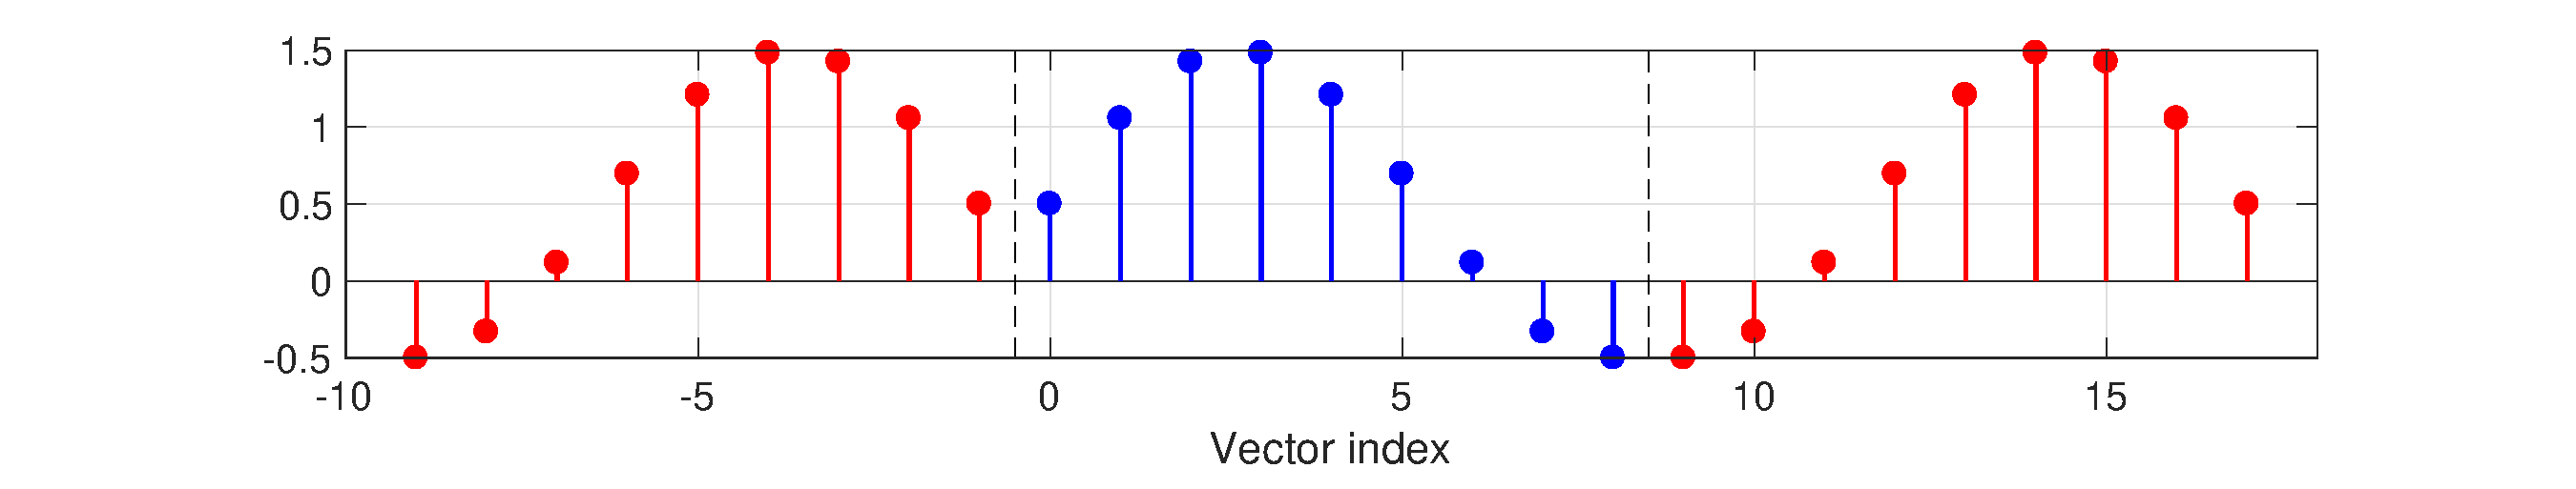
\includegraphics[scale=0.25]{Figures/NeumannBC.eps}
\end{figure}
Letting $J$ be the reversal matrix, the system $\gVec = T_{l}\fVec_{l} + T\fVec + T_{r}\fVec_{r}$ becomes
\[\gVec = [(\mathbf{0}~|~T_{l})J + T + (T_{r}~|~\mathbf{0})J]\fVec = A\fVec,\]
where $\mathbf{0}$ is a zero matrix and $A$ is a Toeplitz-plus-Hankel matrix.
\begin{itemize}
\item When the kernel $\kVec$ is symmetric, $A$ is diagonalized by the DCT \cite{Martucci1994,NeumannDCT}
\item For two-dimensional problems, the corresponding system matrices are block Toeplitz-plus-Hankel with Toeplitz-plus-Hankel blocks \cite{NeumannDCT}
\end{itemize}
\end{frame}

\begin{frame}
\frametitle{Definition of the DCT}
There are eight versions of the DCT, each corresponding to how the left and right endpoints of an interval are handled \cite[p.~36-39]{GolubVanLoan2013}
\begin{block}{DCT-II}
Given $\mathbf{x} \in \mathbb{R}^n$, the DCT-II of $\mathbf{x}$, denoted $\dct{\mathbf{x}}$, is defined as
\[\dct{x}_j = \sum_{k=0}^{n-1} x_k\cos\left(\frac{\pi{j}(2k + 1)}{2n}\right).\]
\end{block}
The DCT has an orthogonal matrix representation $C$ with components
\[C_{j,k} = \sqrt{\frac{2 - \delta_{j,0}}{n}} \cos\left(\frac{\pi{j}(2k + 1)}{2n}\right), 0 \leq j,k \leq n-1.\]
\end{frame}

\begin{frame}
\frametitle{Properties of the DCT}
\begin{itemize}[nosep]
\item The DCT only requires real operations and is thus about twice as fast to use as the DFT \cite{RaoYip2014} 
\item Makhoul \cite{Makhoul1980} described ways of calculating the DCT via the DFT
\item The following are some DCT basis vectors, which are the rows of (non-orthogonal) DCT matrix
\end{itemize}
\begin{center}
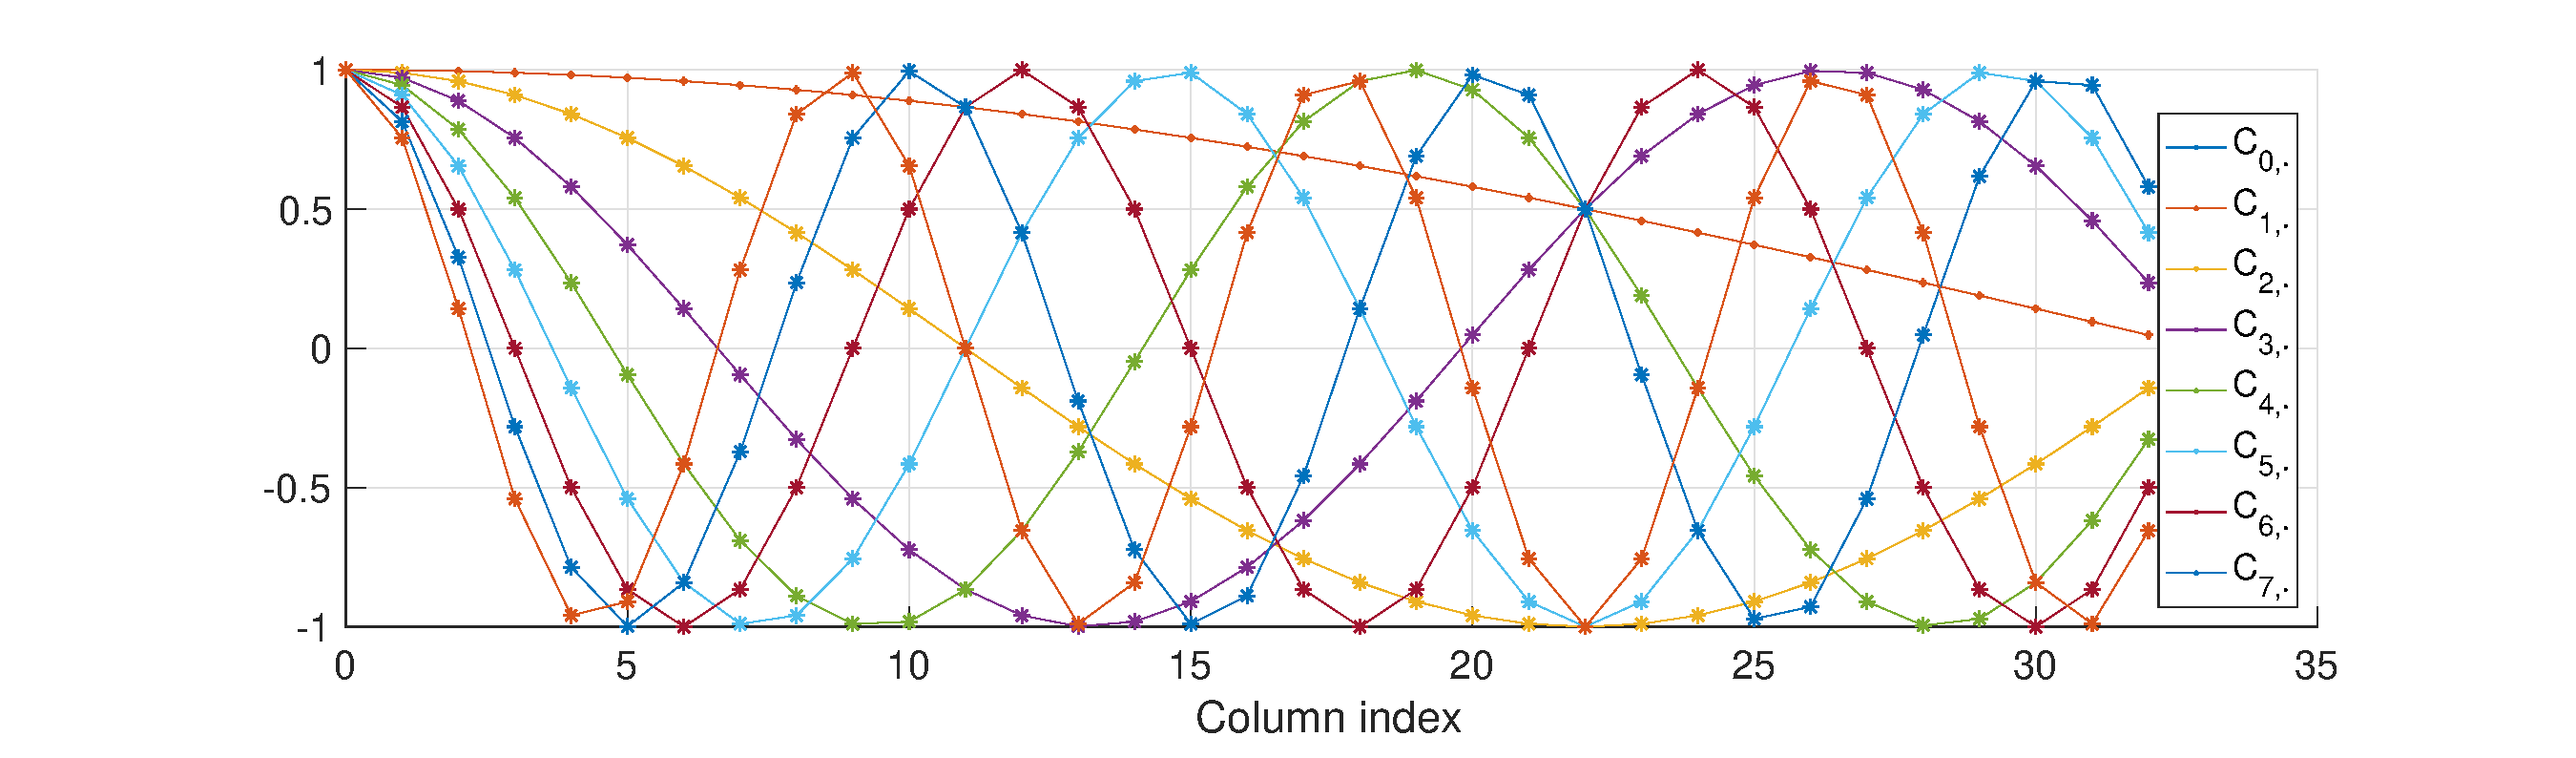
\includegraphics[scale=0.27]{Figures/DCT_Vectors.eps}
\end{center}
\end{frame}

\begin{frame}
\frametitle{Two-dimensional DCT}
  \begin{itemize}
   \item All eight of the DCTs can be expressed as two-dimensional transforms
   \item Two-dimensional DCT matrices can be expressed as $C_m \otimes C_n$ where $C_m$ and $C_n$ are $m \times m$ and $n \times n$ DCT matrices, respectively
   \item Below are examples of the two-dimensional DCT basis vectors
  \end{itemize}
 \begin{center}
  \includegraphics[scale=0.4]{Figures/DCT-8x8.png}
 \end{center}
\end{frame}

\begin{frame}
\frametitle{DCT-version of UPRE}
If $K = C^\trans\Delta{C}$ and $D = C^\trans\Lambda{C}$ (see \cite{Strang1999}), then
\[\frac{1}{n}\|\regres\|^2 = \frac{1}{n}\|C\regres\|^2 = \frac{1}{n}\|C(C^\trans\Delta{C})\regf - C\gnoiseVec\|^2 = \frac{1}{n}\|\Delta\dct{\regf} - \dct{\gnoiseVec}\|^2.\]
Thus the product $\Delta\dct{\regf}$ can be written as
\[\Delta\dct{\regf} = \Delta{C}[(K^\trans{K} + \regparam{D^\trans}D)^{-1}C^\trans\gnoiseVec] = \Delta(\Delta^\trans{\Delta} + \regparam\Lambda^\trans{\Lambda})^{-1}\Delta^\trans\dct{\gnoiseVec}.\]
Therefore
\begin{align*}
\frac{1}{n}\|\regres\|^2 &= \frac{1}{n}\|\Delta(\Delta^\trans{\Delta} + \regparam\Lambda^\trans{\Lambda})^{-1}\Delta^\trans\dct{\gnoiseVec} - \dct{\gnoiseVec}\|^2 \\
&= \frac{1}{n}\|(\Delta(\Delta^\trans{\Delta} + \regparam\Lambda^\trans{\Lambda})^{-1}\Delta^\trans - I)\dct{\gnoiseVec}\|^2.
\end{align*}
If $D = I$, then
\[\frac{1}{n}\|\regres\|^2 = \frac{1}{n}\sum_{j=0}^{n-1}(\dct{\gnoise}_j)^2\left(\mfilt(\regparam,\dct{k}_j)\right)^2.\]
\end{frame}

\begin{frame}
\frametitle{DCT-version of UPRE}
The Tikhonov influence matrix $\A$ can be expressed as
\[\A = K(K^\trans{K} + \regparam{D^\ctrans}D)^{-1}K^\ctrans = C^\trans\Delta(\Delta^\trans{D} + \regparam\Lambda^\ctrans{\Lambda})^{-1}\Delta^\trans{C}.\]
Since $\Delta(\Delta^\trans{D} + \regparam\Lambda^\trans{\Lambda})^{-1}\Delta^\trans$ is diagonal, if $D = I$ then
\[\trace(\A) = \sum_{j = 0}^{n-1} \frac{(\dct{k}_j)^2}{(\dct{k}_j)^2 + \regparam(\dct{d}_j)^2} = \sum_{j = 0}^{n-1} \filt(\regparam,\dct{k}_j).\]
\begin{block}{DCT-version of the UPRE function}
Under the assumptions that $K$ is diagonalized by the DCT and that $D = I$,
\[\U_n(\regparam) = \frac{1}{n}\sum_{j = 0}^{n-1} (\dct{\gnoise}_j)^2(\mfilt(\regparam,\dct{k}_j))^2 + \frac{2\noiseSD^2}{n}\sum_{j = 0}^{n-1} \filt(\regparam,\dct{k}_j) - \noiseSD^2.\]
\end{block}
\end{frame}

\begin{frame}
\frametitle{Statistics of the UPRE}
Under the assumption that $\mathbf{\noiseVec} \sim \mathcal{N}(\mathbf{0},\noiseSD^2 I)$, the orthogonality of the DCT matrix $C$ produces
\[C\mathbf{\gnoiseVec} = \dct{\mathbf{\gnoiseVec}} \sim \mathcal{N}(C\mathbf{\gVec},\noiseSD^2 CC^\trans) = \mathcal{N}(\dct{\mathbf{\gVec}},\noiseSD^2 I).\]
Thus statistical results like the following can be obtained.
\begin{block}{Expected value of $\U_n(\regparam)$}
\begin{align*}
\E\left(\U_n(\regparam)\right) &= \frac{1}{n}\sum_{j = 0}^{n-1} \E\left((\dct{\gnoise}_j)^2\right)(\mfilt(\regparam,\dct{k}_j))^2 + \frac{2\noiseSD^2}{n}\sum_{j = 0}^{n-1} \filt(\regparam,\dct{k}_j) - \noiseSD^2 \\
&= \frac{1}{n}\sum_{j = 0}^{n-1} \frac{\noiseSD^2}{2}\left(2 + \frac{(\dct{g}_j)^2}{\noiseSD^2}\right)(\mfilt(\regparam,\dct{k}_j))^2 + \frac{2\noiseSD^2}{n}\sum_{j = 0}^{n-1} \filt(\regparam,\dct{k}_j) - \noiseSD^2
\end{align*}
\end{block}
Recently similar statistical results for the UPRE were used to bound the location of minimizers of $\U_n(\regparam)$ \cite{RenautHelmstetterVatankhah}.
\end{frame}

\begin{frame}
\frametitle{DCT-version of GCV and the discrepancy principle}
Since both the GCV and discrepancy principle functions use $\frac{1}{n}\|\regres\|^2$, their DCT-versions are readily obtained.
\begin{block}{DCT-version of the GCV function}
Under the assumptions that $K$ is diagonalized by the DCT and that $D = I$,
\[\GCV_n(\regparam) = \frac{n \sum_{j = 0}^{n-1} |\dct{\gnoise}_j|^2(\mfilt(\regparam,|\dct{k}_j|))^2}{(\sum_{j = 0}^{n-1} \mfilt(\regparam,|\dct{k}_j|))^2}.\]
\end{block}
\begin{block}{DCT-version of the discrepancy principle function}
Under the assumptions that $K$ is diagonalized by the DCT and that $D = I$,
\[\D_n(\regparam) = \sum_{j = 0}^{n-1} |\dct{\gnoise}_j|^2(\mfilt(\regparam,|\dct{k}_j|))^2 - \noiseSD^2.\]
\end{block}
\end{frame}

\begin{frame}
\frametitle{Numerical results using the DCT}
\begin{figure}
\centering
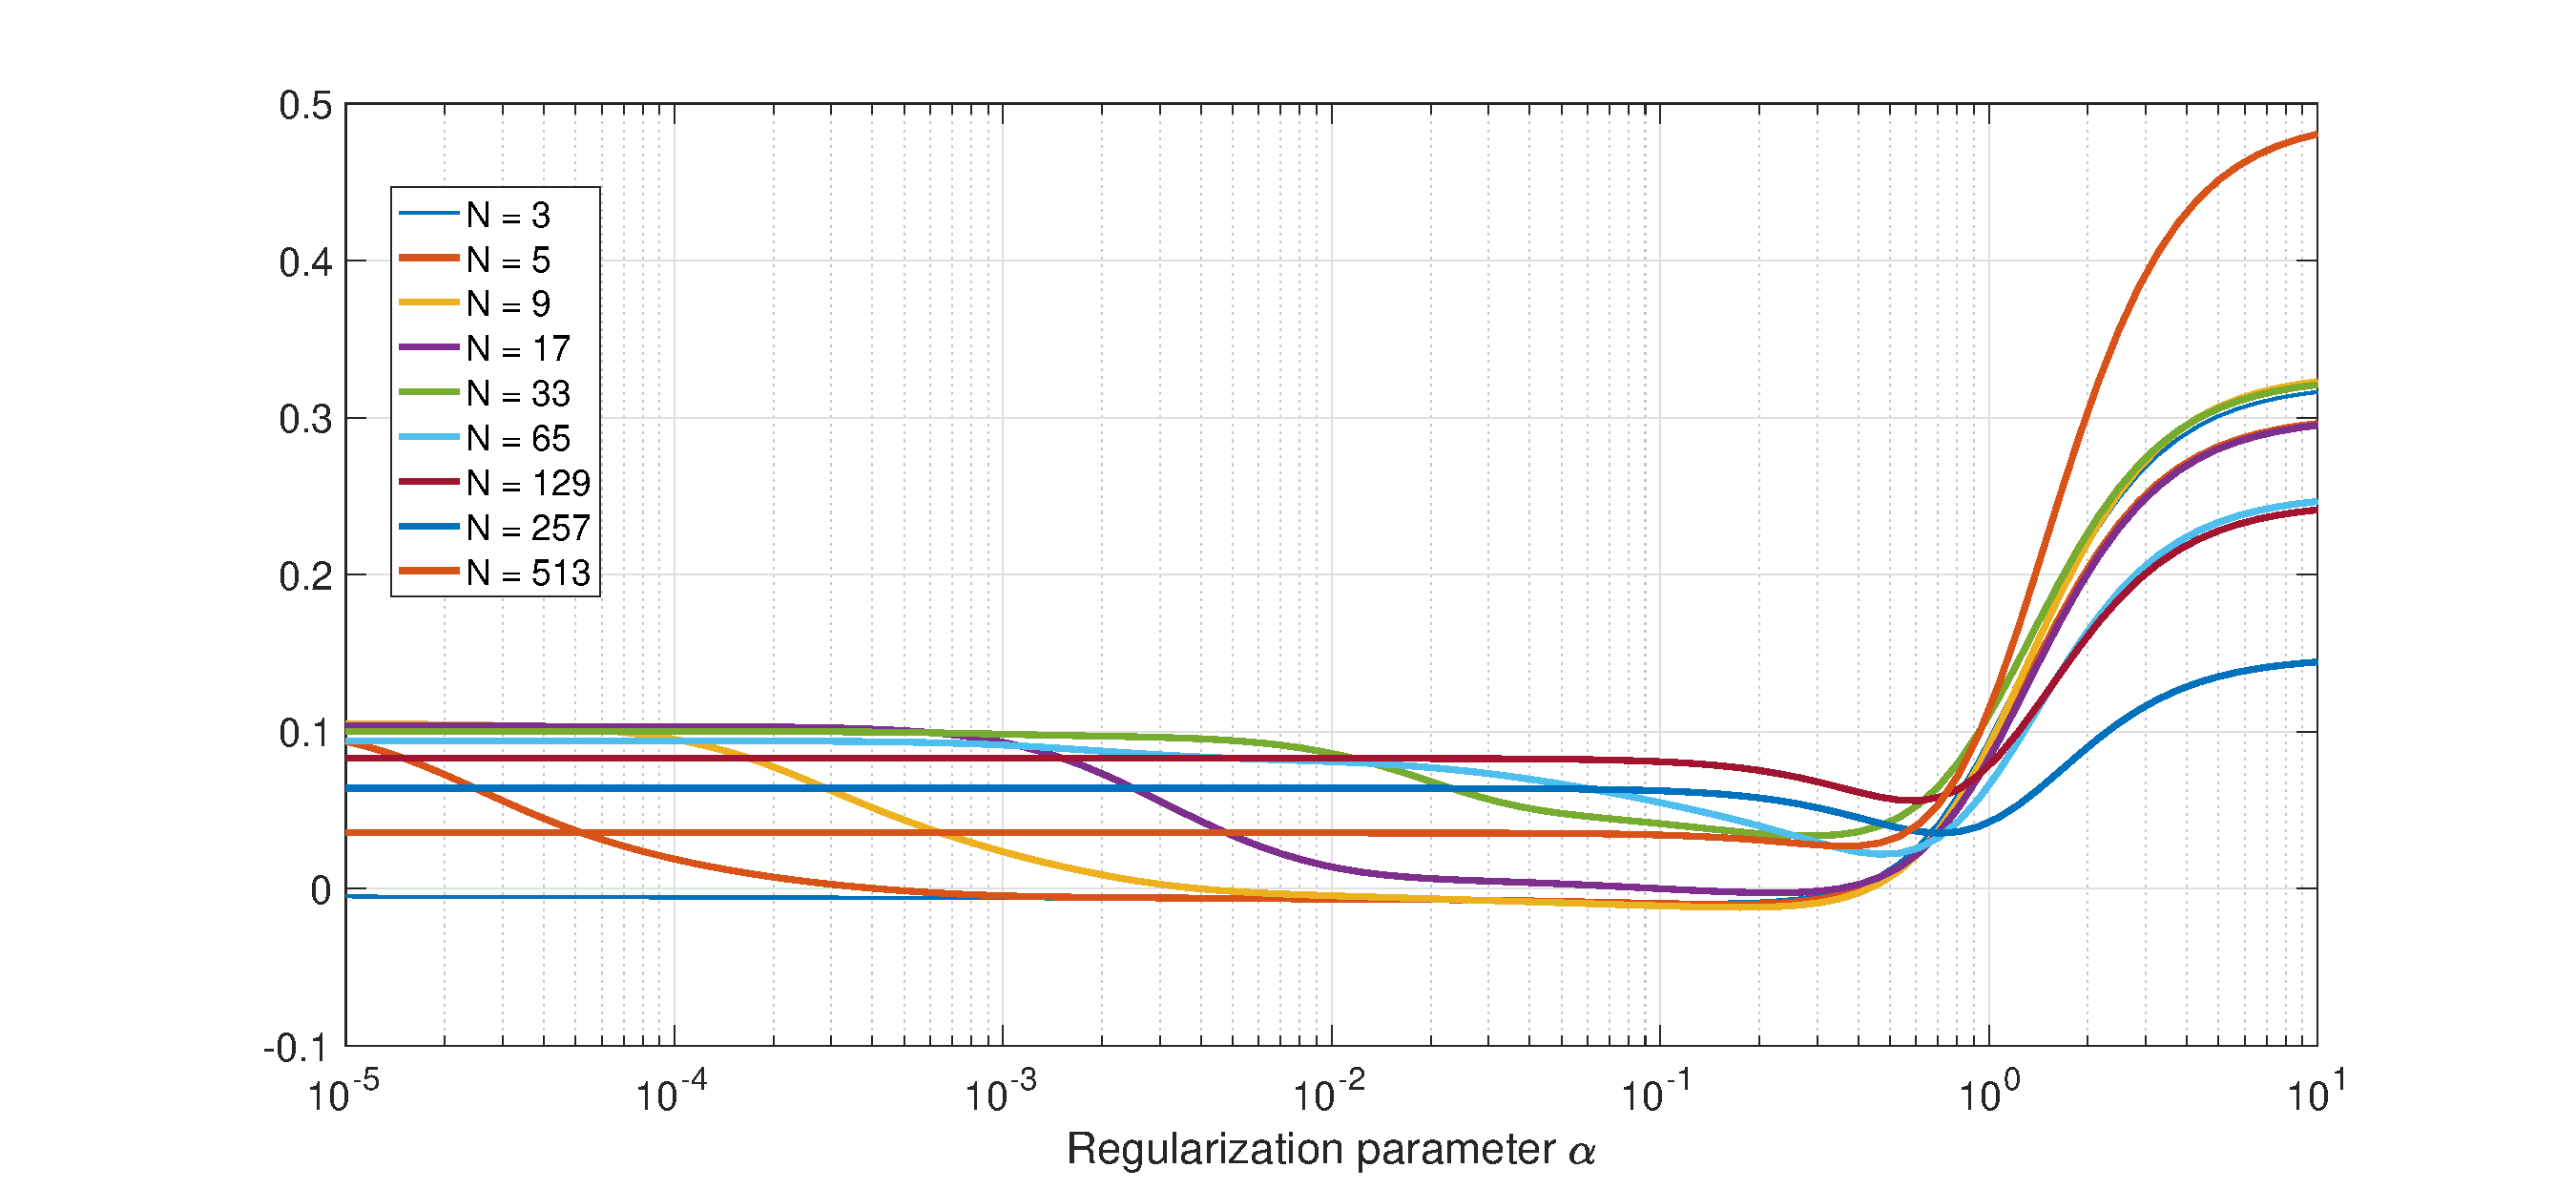
\includegraphics[scale=0.25]{Figures/UPRE_Vec.eps}
\caption{Graphs of UPRE functions for various downsampling levels. The width parameter of the Gaussian kernel was 200 and the SNR was 5.}
\end{figure}
\end{frame}

\begin{frame}
\frametitle{Numerical results using the DCT}
\begin{figure}
\centering
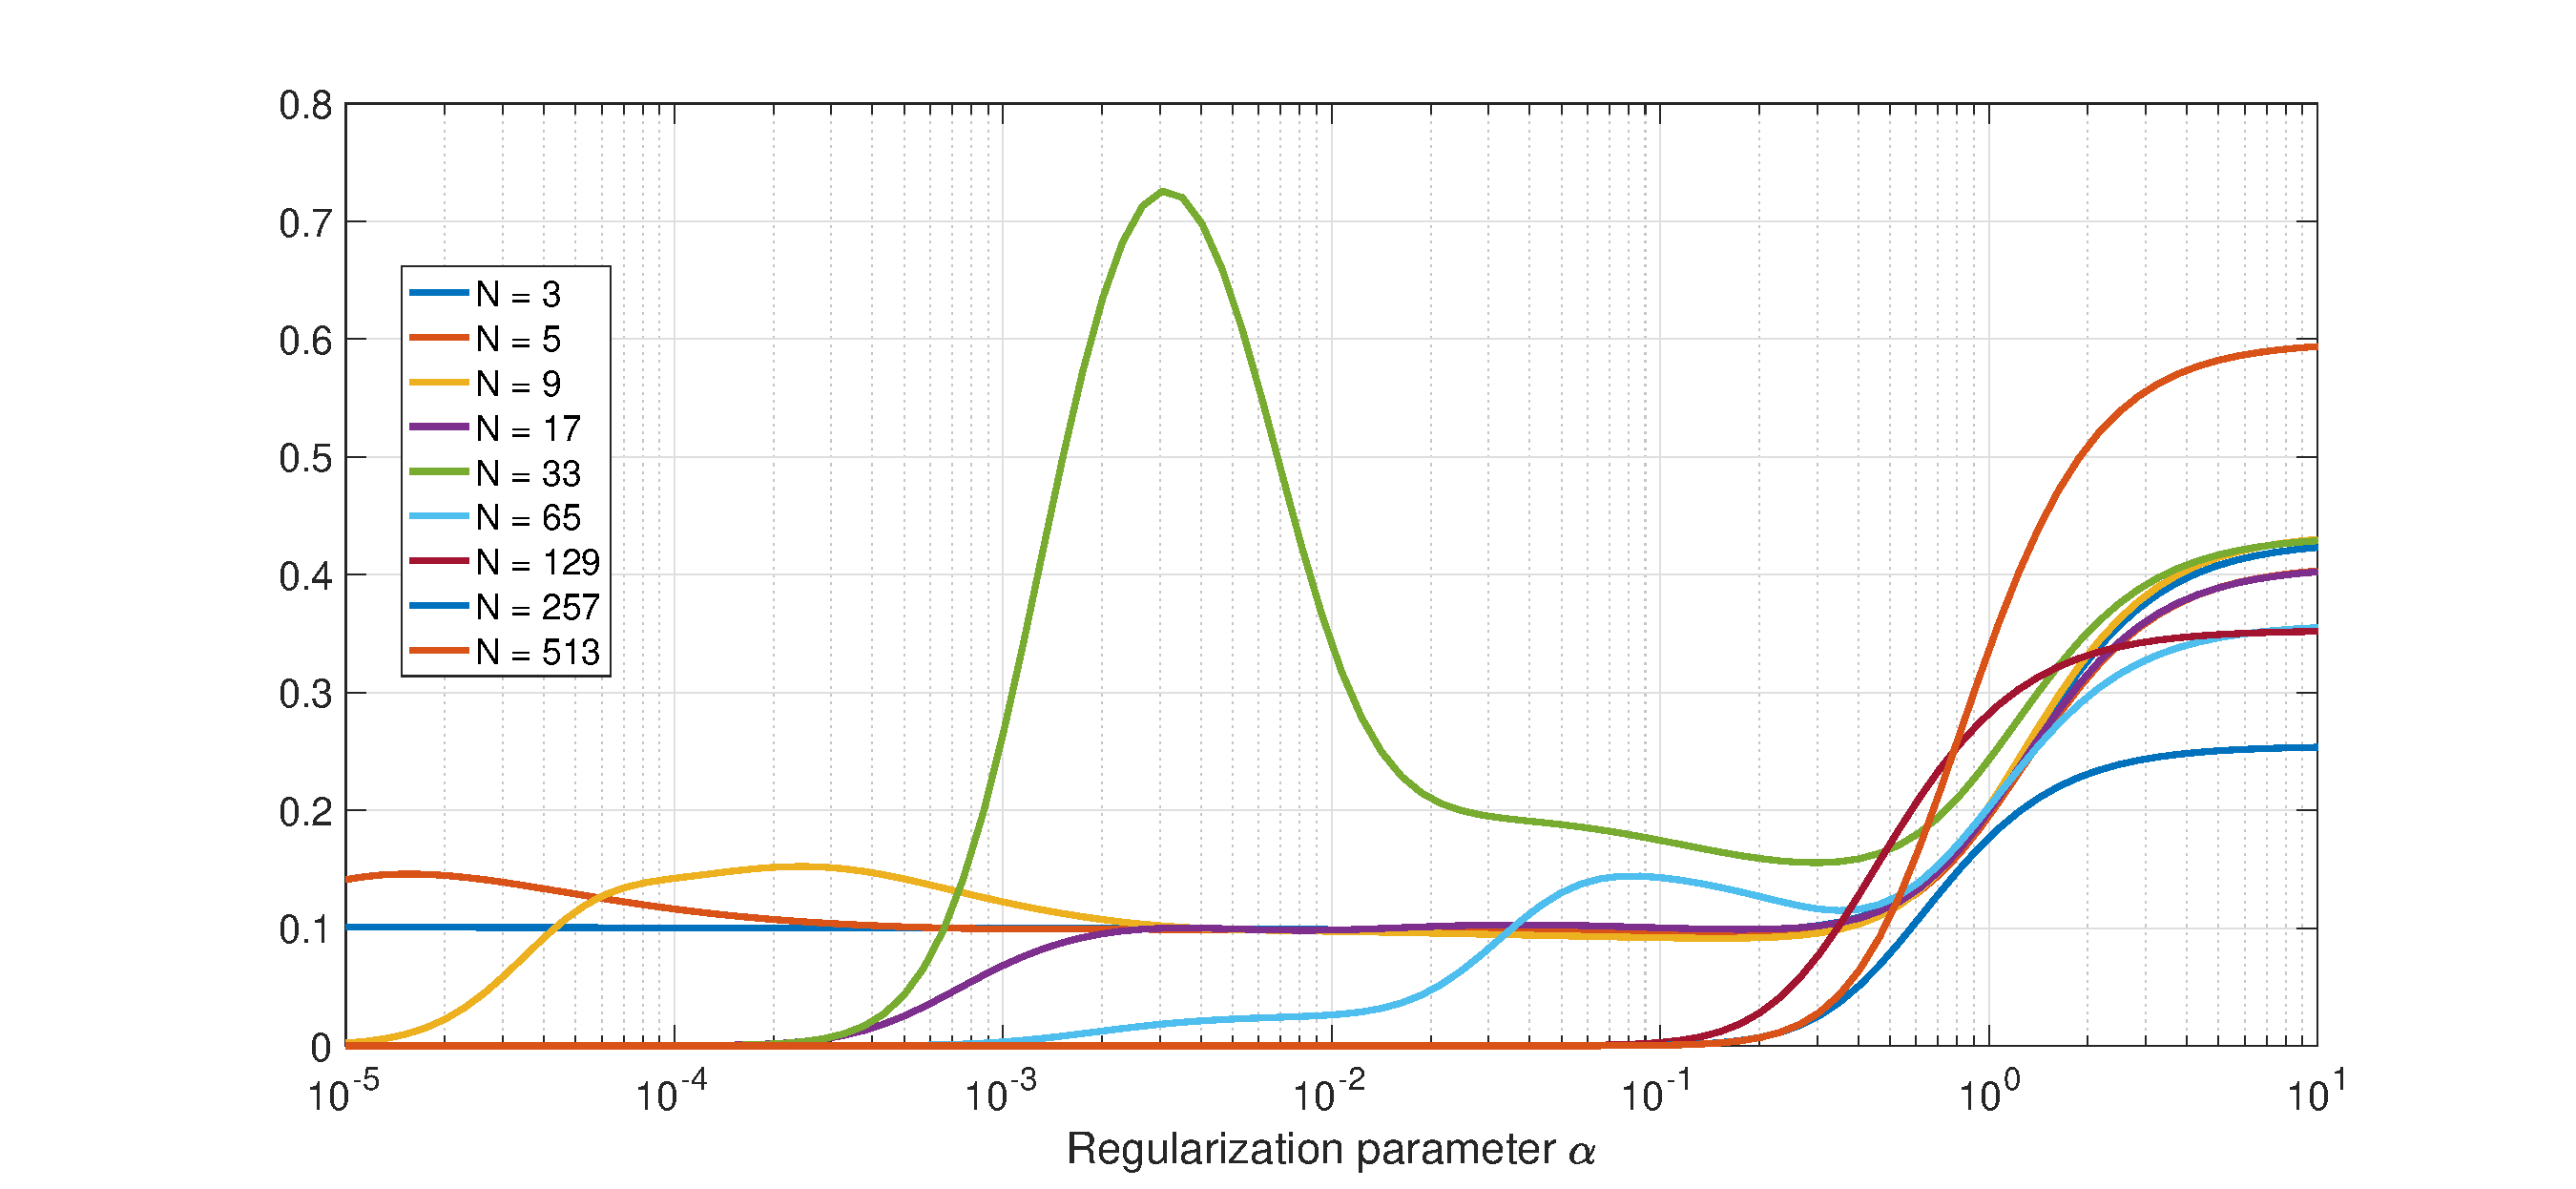
\includegraphics[scale=0.25]{Figures/GCV_Vec.eps}
\caption{Graphs of GCV functions for various downsampling levels. The width parameter of the Gaussian kernel was 200 and the SNR was 5.}
\end{figure}
\end{frame}

\begin{frame}
\frametitle{Numerical results using the DCT}
\begin{figure}
\centering
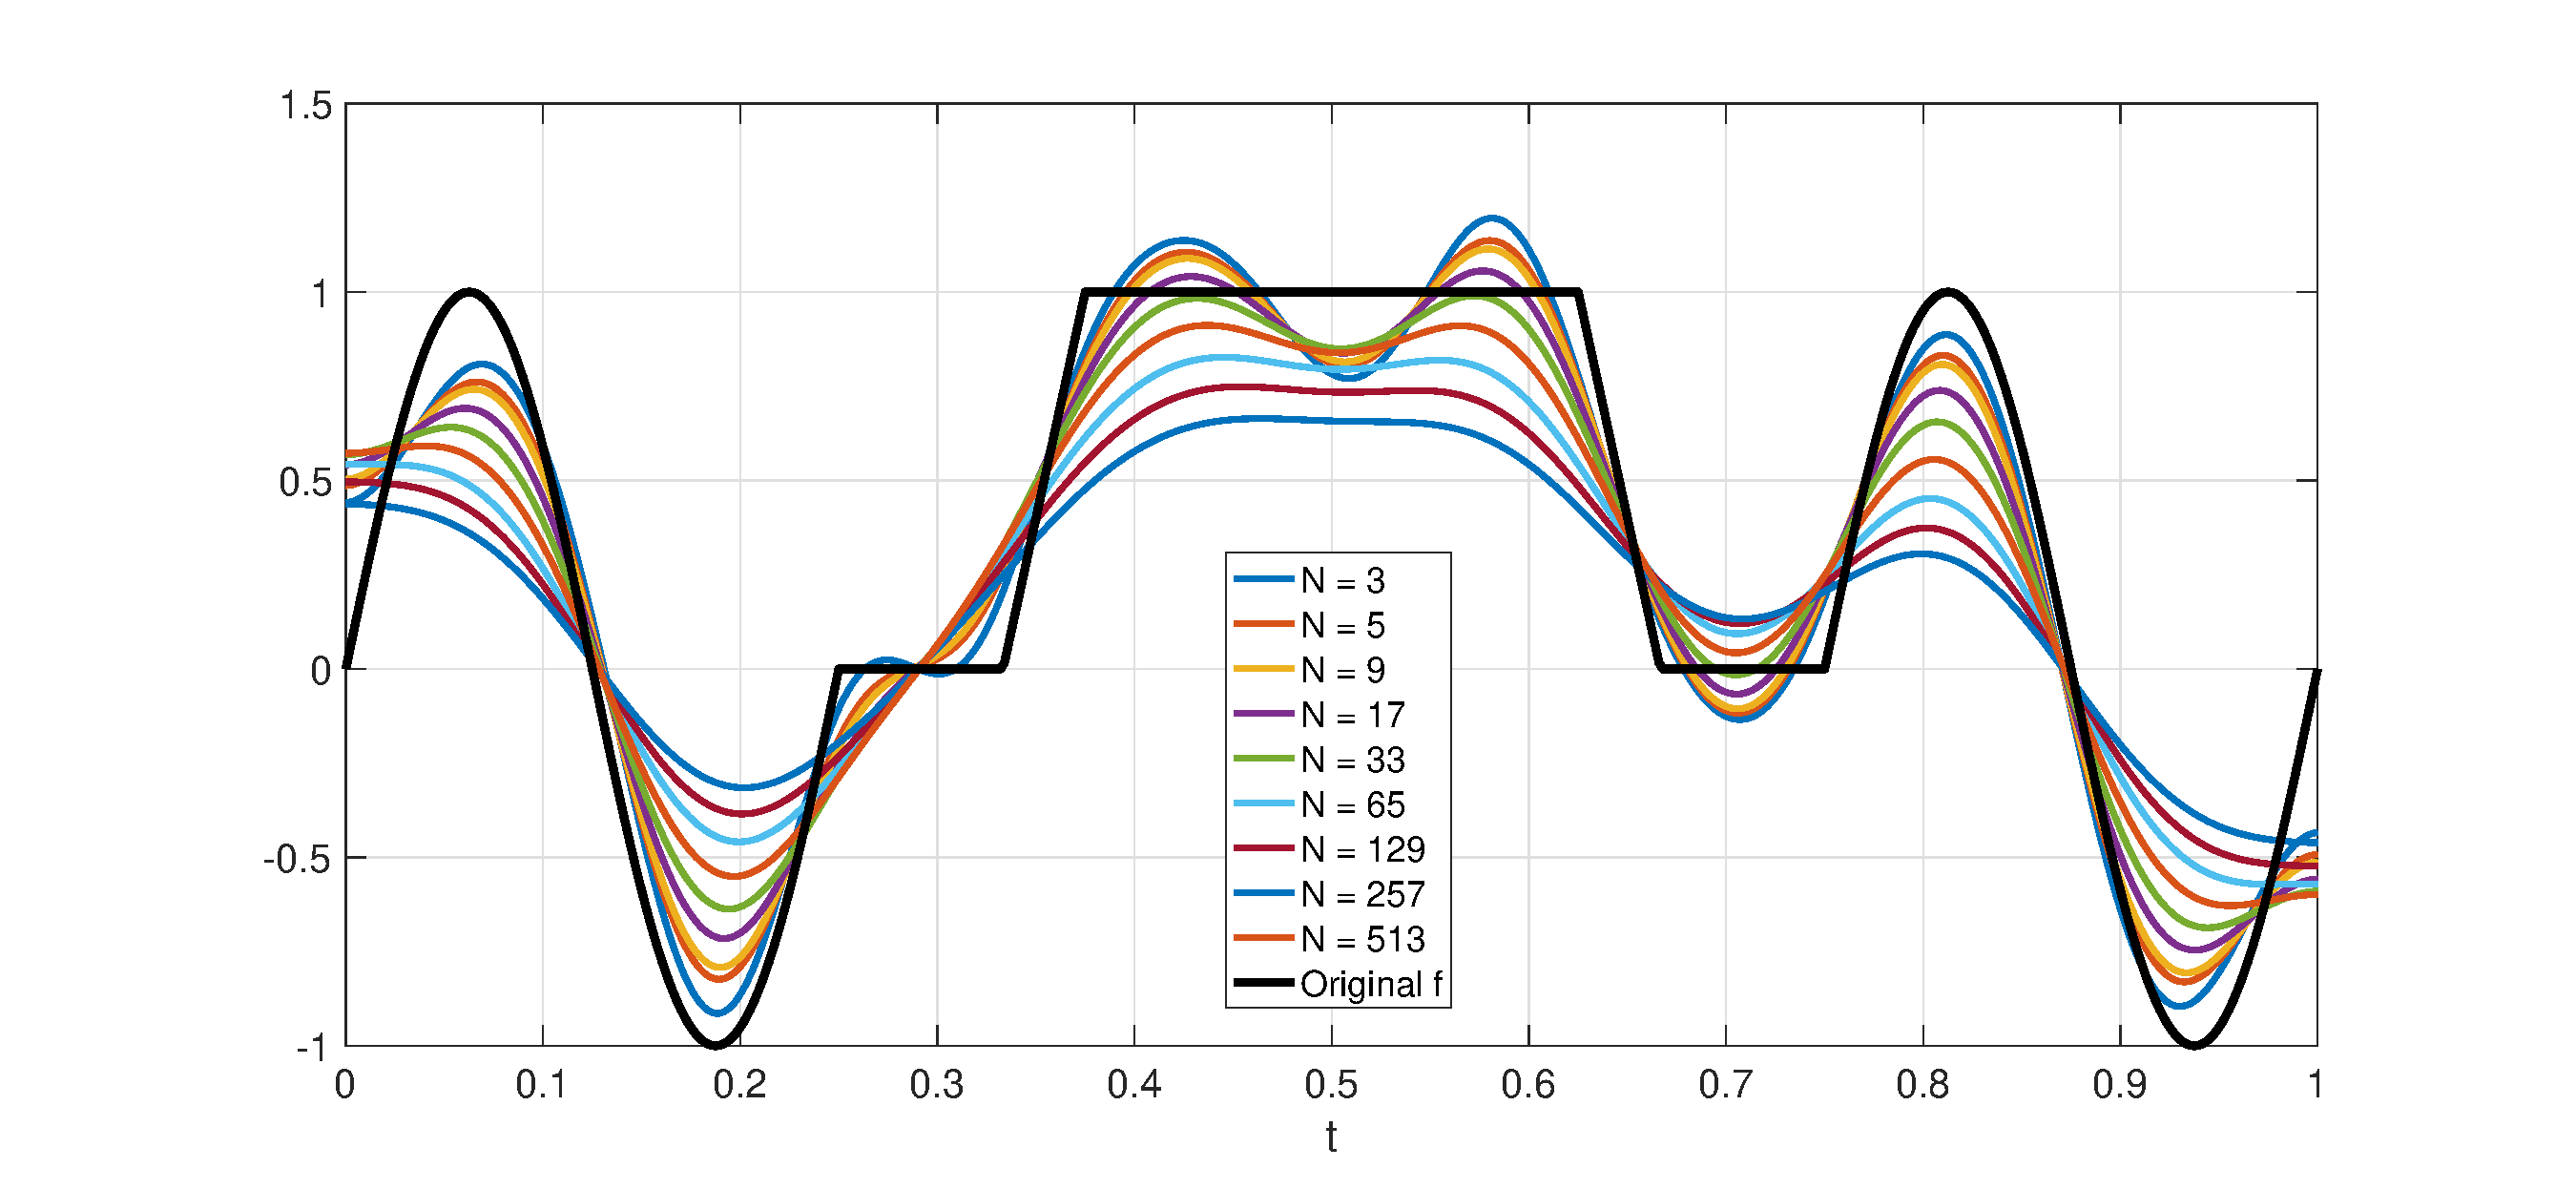
\includegraphics[scale=0.25]{Figures/UPRE_Sols.eps}
\caption{Graphs of the solutions obtained by Tikhonov regularization, where the regularization parameter was selected using the UPRE method. The width of the Gaussian kernel was 200 and the SNR was 25.}
\end{figure}
\end{frame}

\begin{frame}
\frametitle{Numerical results using the DCT}
\begin{figure}
\centering
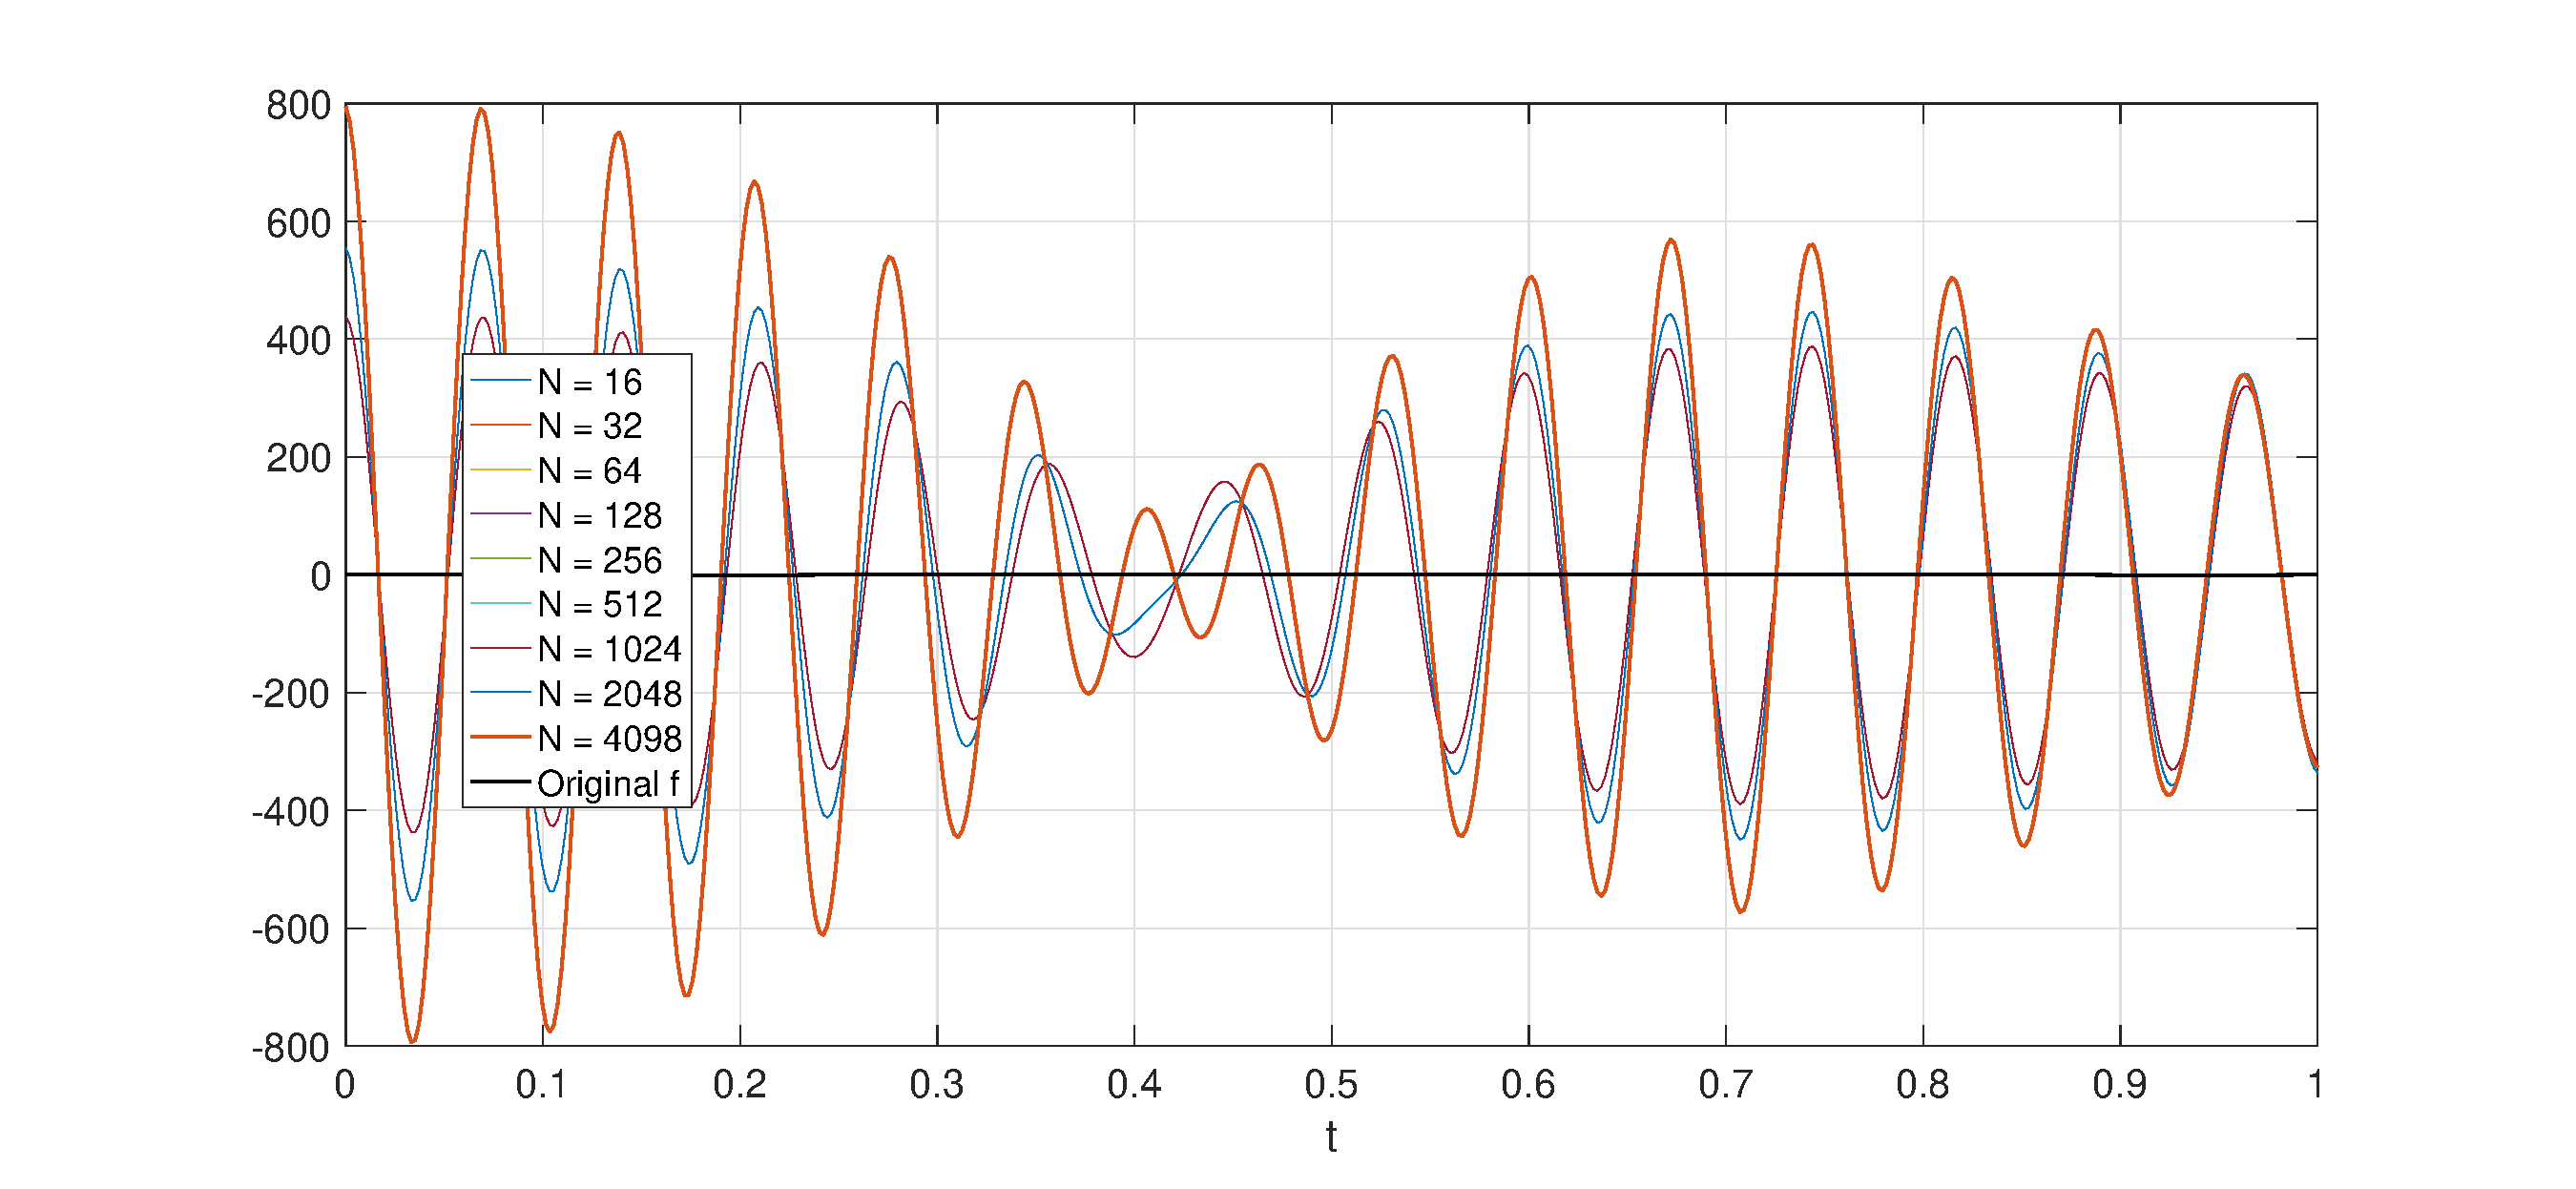
\includegraphics[scale=0.25]{Figures/GCV_Sols.eps}
\caption{Graphs of the solutions obtained by Tikhonov regularization, where the regularization parameter was selected using the GCV method. The width of the Gaussian kernel was 200 and the SNR was 25.}
\end{figure}
\end{frame}

\begin{frame}
\frametitle{Numerical results using the DCT}
\begin{figure}
\centering
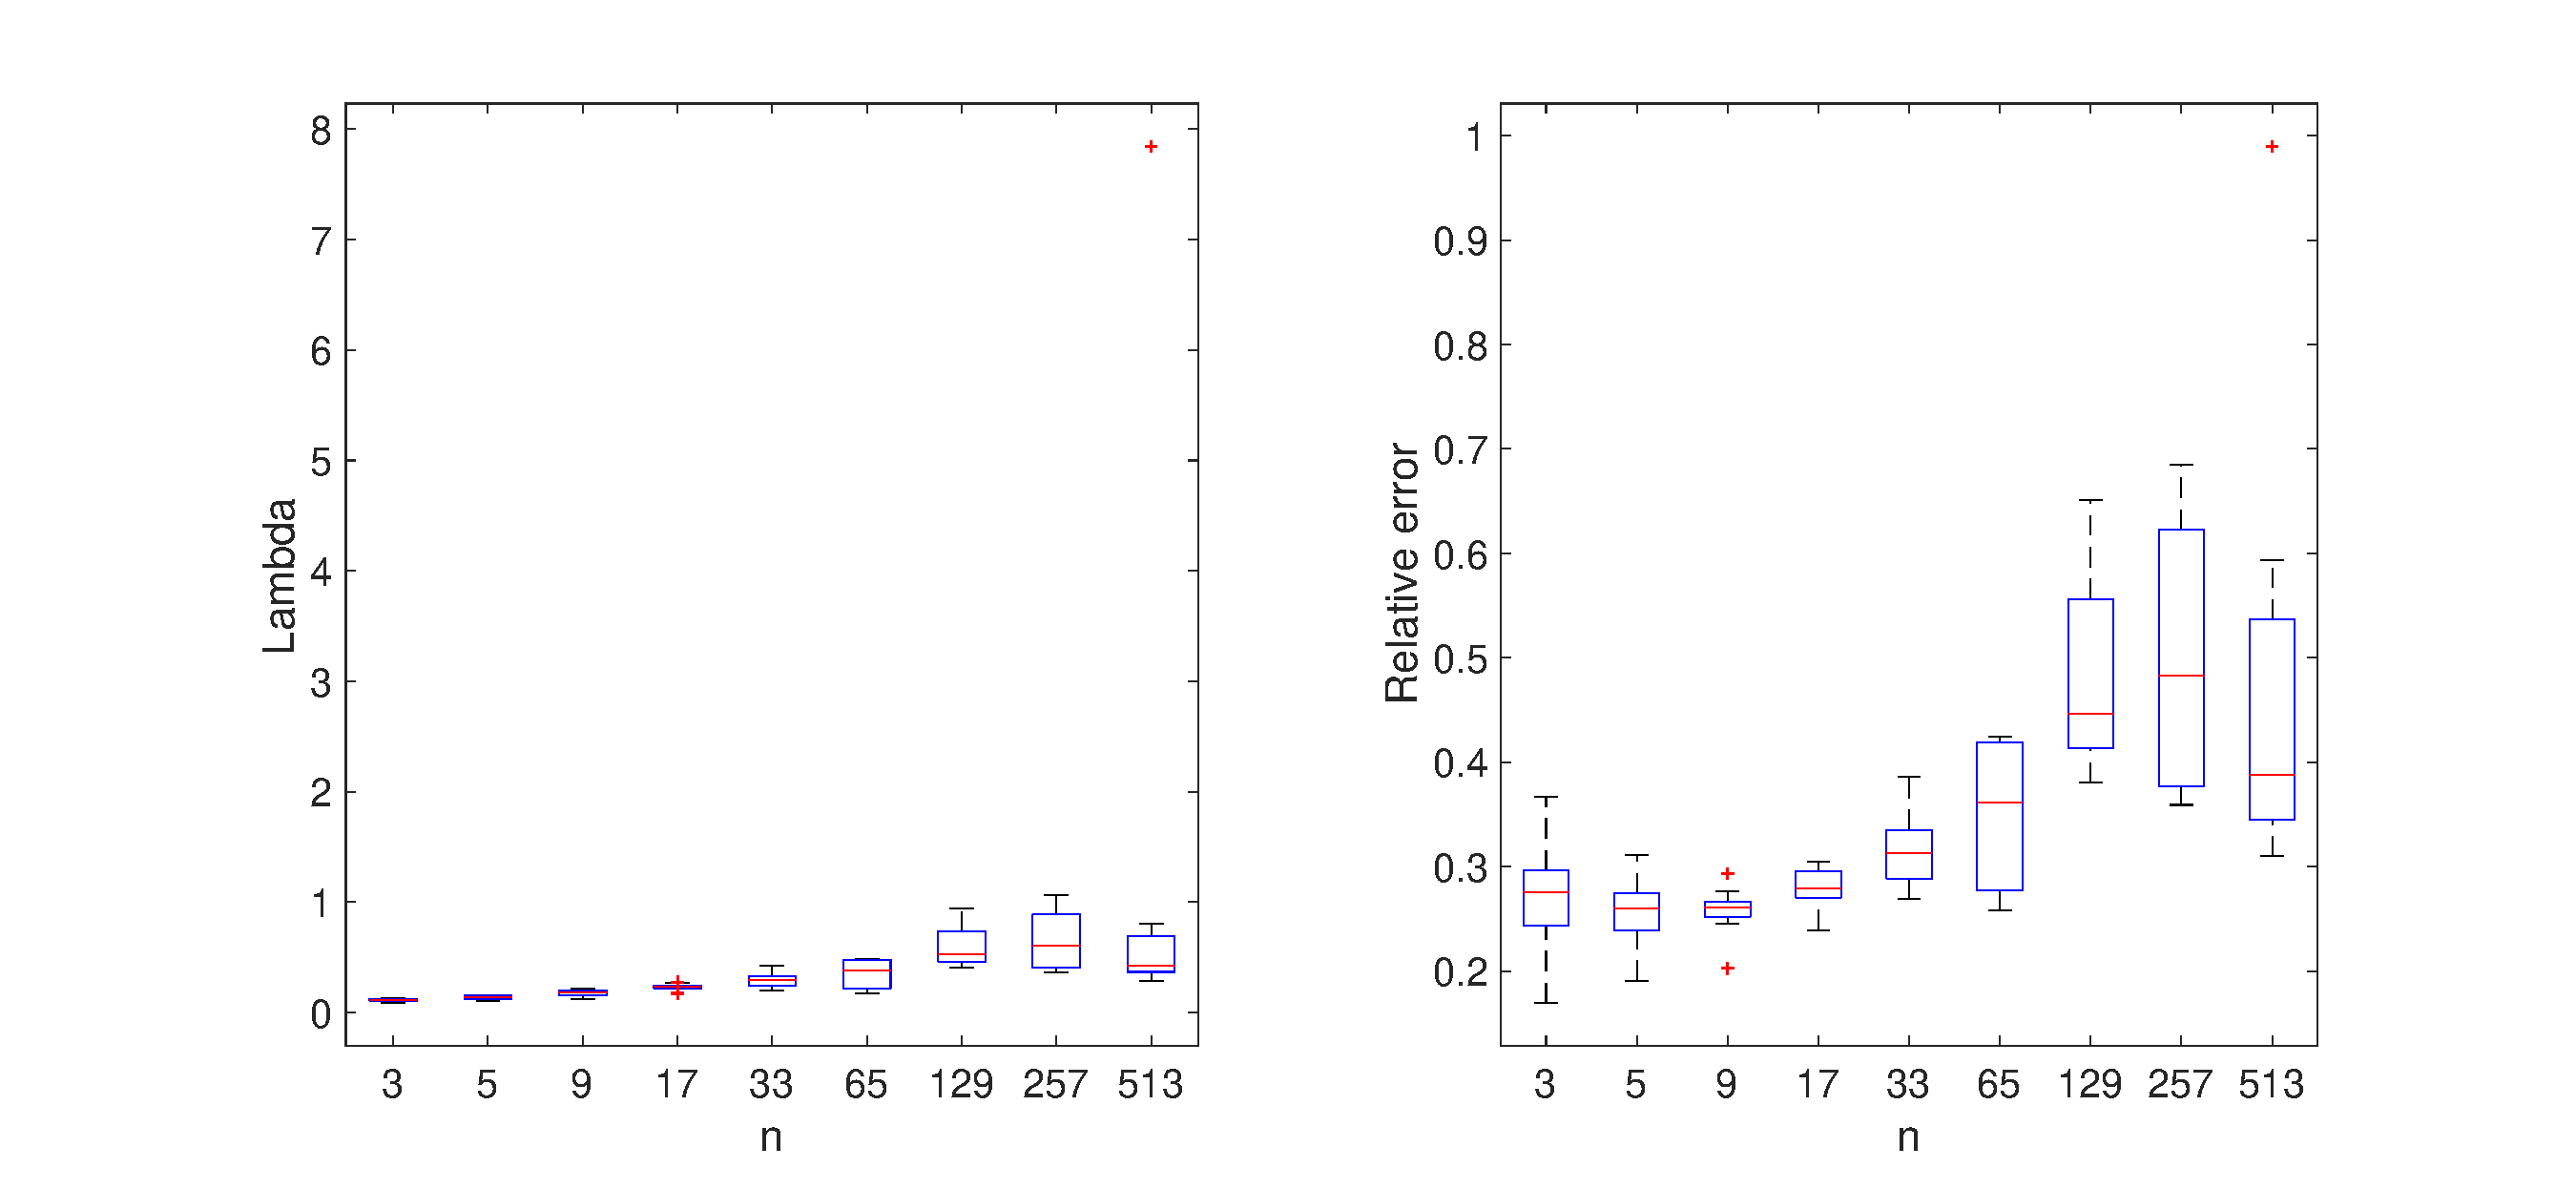
\includegraphics[scale=0.25]{Figures/UPRE_Boxes.eps}
\caption{(Left) Boxplot showing the variability of selected regularization parameters using the UPRE method with 10 noise realization. The test problem involved an SNR of 5 and the width of the Gaussian kernel was 200. (Right) Boxplot showing the variability of the relative errors of the regularized solutions.}
\end{figure}
\end{frame}

\section{DFT approach}

\begin{frame}
\frametitle{Periodic boundary condition}
\begin{figure}
\centering
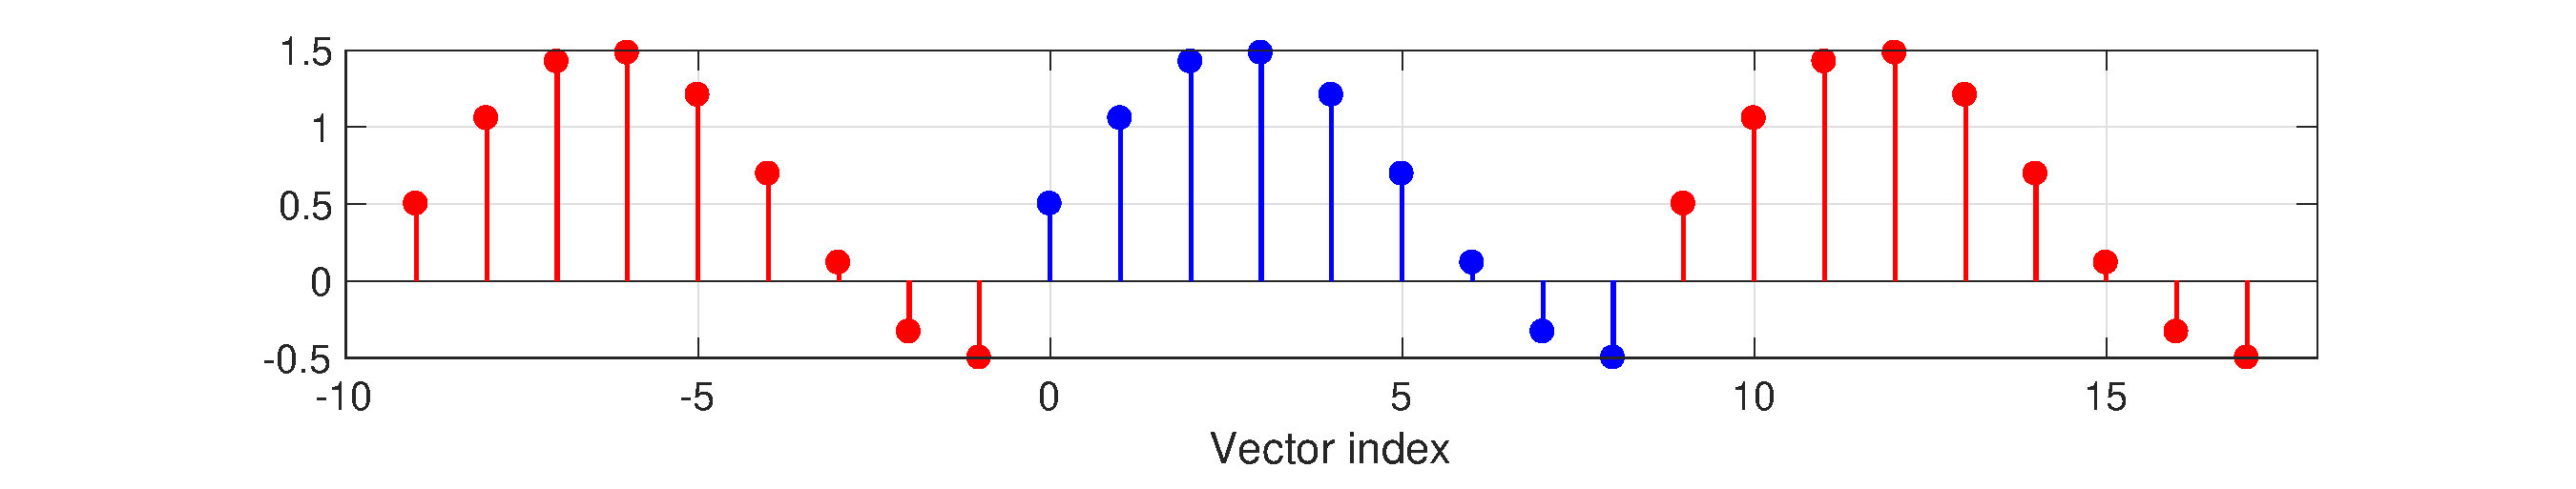
\includegraphics[scale=0.25]{Figures/PeriodicBC.eps}
\end{figure}
Letting $J$ be the reversal matrix, the system $\gVec = T_{l}\fVec_{l} + T\fVec + T_{r}\fVec_{r}$ becomes
\[\gVec = [(\mathbf{0}~|~T_{l}) + T + (T_{r}~|~\mathbf{0})]\fVec = B\fVec,\]
where $\mathbf{0}$ is a zero matrix and $B$ is a circulant matrix.
\begin{itemize}
\item Circulant matrices are diagonalized by the DFT
\item For two-dimensional problems, the corresponding system matrices are block circulant with circulant blocks (BCCB) \cite{Vogel:2002}
\item Due to the fast Fourier transform (FFT), the cost of using the DFT is $O(n\log(n))$ instead of $O(n^2)$ \cite{CooleyTukey}
\end{itemize}
\end{frame}

\begin{frame}
\frametitle{Definition of the DFT}
\begin{block}{The discrete Fourier transform}
Given $\mathbf{x} \in \mathbb{C}^n$, the DFT of $\mathbf{x}$, denoted $\widehat{\mathbf{x}}$, is defined as
\[\widehat{x}_j = \frac{1}{n} \sum_{k=0}^{n-1} x_k\exp\left(\frac{-2\pi{ijk}}{n}\right).\]
\end{block}
The DFT has a unitary matrix representation $F$ with components
\[F_{j,k} = \frac{1}{\sqrt{n}}\exp\left(\frac{-2\pi{ijk}}{n}\right), 0 \leq j,k \leq n-1.\]
Using $F$, a circulant matrix $B$ has the decomposition
\[B = F^\ctrans\Delta{F},\]
where $\Delta  = \diag(\sqrt{n}\widehat{\mathbf{b}})$ and $\widehat{\mathbf{b}} = FB_{\cdot,0}$ \cite[p.~69]{Vogel:2002}.
\end{frame}

\begin{frame}
\frametitle{DFT-versions of parameter estimation functions}
If $K$ is circulant and $D = I$, then we have the following.
\begin{block}{DFT-version of the UPRE function}
\[\U_n(\regparam) = \frac{1}{n}\sum_{j = 0}^{n-1} |\widehat{\gnoise}_j|^2(\mfilt(\regparam,|\widehat{k}_j|))^2 + \frac{2\noiseSD^2}{n}\sum_{j = 0}^{n-1} \filt(\regparam,|\widehat{k}_j|) - \noiseSD^2.\]
\end{block}
\begin{block}{DFT-version of the GCV function}
\[\GCV_n(\regparam) = \frac{n \sum_{j = 0}^{n-1} |\widehat{\gnoise}_j|^2(\mfilt(\regparam,|\widehat{k}_j|))^2}{(\sum_{j = 0}^{n-1} \mfilt(\regparam,|\widehat{k}_j|))^2}.\]
\end{block}
\begin{block}{DFT-version of the discrepancy principle function}
\[\D_n(\regparam) = \sum_{j = 0}^{n-1} |\widehat{\gnoise}_j|^2(\mfilt(\regparam,|\widehat{k}_j|))^2 - \noiseSD^2.\]
\end{block}
\end{frame}

\begin{frame}
\frametitle{Statistics involving the DFT}
Since $F : \mathbb{C}^n \rightarrow \mathbb{C}^n$, if $\mathbf{\noiseVec} \sim \mathcal{N}(\mathbf{0},\noiseSD^2 I)$ then $F\mathbf{\noiseVec} = \widehat{\mathbf{\noiseVec}}$ does not have a probability density function in the traditional sense.
\begin{itemize}
\item Arises from the fact that $AA^\trans$ and $BB^\trans$, where $A = \Re(F)$ and $B = \Im(F)$, are rank-deficient
\item Probability density functions for $\Re(\widehat{\mathbf{\noiseVec}})$ and $\Im(\widehat{\mathbf{\noiseVec}})$ exist on $\rank(AA^\trans)$ and $\rank(BB^\trans)$-dimensional subspaces, respectively \cite[p.~527-528]{Rao1973}
\end{itemize}
Instead, distributions of the components of $\widehat{\mathbf{\noiseVec}}$ can be handled individually. Results such as the following are then obtained.
\begin{block}{}
For $\noiseVec \sim \mathcal{N}(\mathbf{0},\noiseSD^2 I)$, let $J = \{0,n/2\}$ if $n$ is even and $J = \{0\}$ if $n$ is odd. Then for $0 \leq j \leq n-1$, the distribution of $|\widehat{\noise}_j|^2 = \Re(\widehat{\noise}_j)^2 + \Im(\widehat{\noise}_j)^2$ is as follows.
\[|\widehat{\noise}_j|^2 \sim \begin{cases}
\text{gamma}(1/2,2\noiseSD^2), & j \in J \\
\text{exponential}(\noiseSD^2), & j \not\in J \end{cases}.\]
\end{block}
\end{frame}

\begin{frame}
\frametitle{Downsampling and the DFT}
Given a vector $\mathbf{x} \in \mathbb{C}^N$ with $N = LM$, the \textit{aliasing operator} $\text{A}_L : \mathbb{C}^N \rightarrow \mathbb{C}^M$ is defined by
\[\left(\text{A}_L(\mathbf{x})\right)_j = \sum_{k=0}^{L-1} x_{j+kM}, \quad \mathbf{x} \in \mathbb{C}^N, \quad 0 \leq j \leq M-1.\]
Letting $\mathbf{x}^M$ be the downsampling of $\mathbf{x}$ formed by every $L$th component of $\mathbf{x}$, the following result relates downsampling and the aliasing operator.
\begin{block}{Downsampling Theorem \cite{AudioDFT}}
Let $\mathbf{x} \in \mathbb{C}^N$, with $N = LM$, let $\mathbf{y} = \mathbf{x}^M$, and let $\widehat{\mathbf{x}}$ and $\widehat{\mathbf{y}}$ denote the DFT of $\mathbf{x}$ and $\mathbf{y}$, respectively. Then
\[\widehat{\mathbf{y}} = \frac{1}{L} \text{A}_L(\widehat{\mathbf{x}}).\]
\end{block}
\end{frame}

\begin{frame}
\frametitle{Numerical results using the DFT}
\begin{figure}
\centering
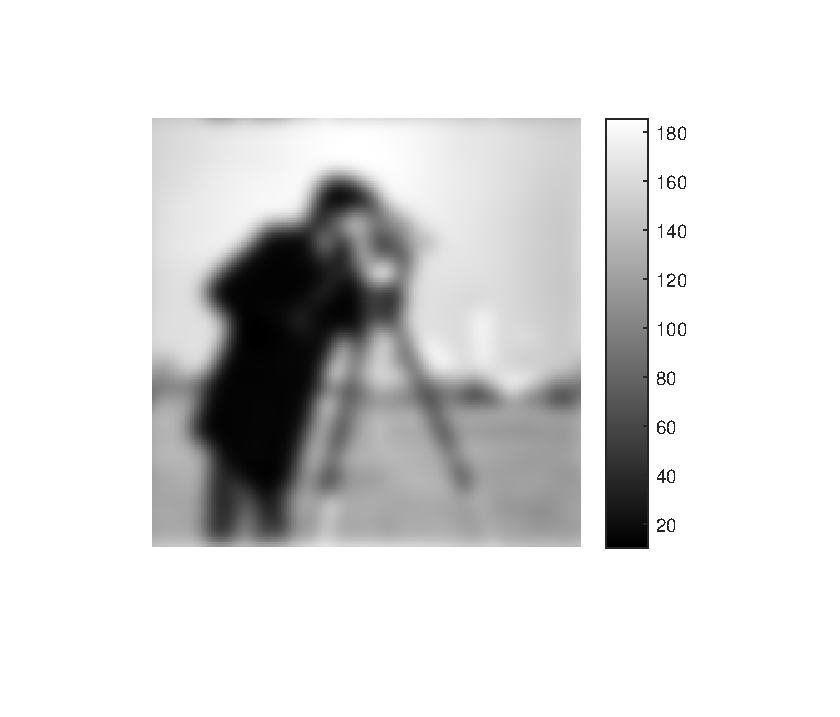
\includegraphics[scale=0.45]{Figures/CameramanBlurred.eps}
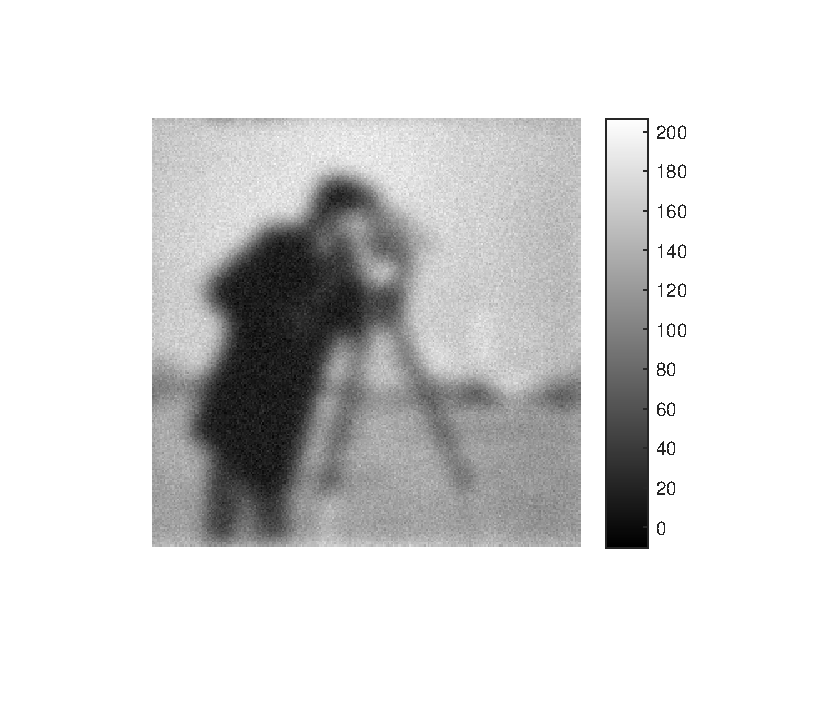
\includegraphics[scale=0.45]{Figures/CameramanBlurredNoisy.eps}
\caption{(Left) Blurred image with Gaussian kernel of width 1000. (Right) The blurred image after the addition of white noise. The image has an SNR of 5.}
\end{figure}
\end{frame}

\begin{frame}
\frametitle{Numerical results using the DFT}
\begin{figure}
\centering
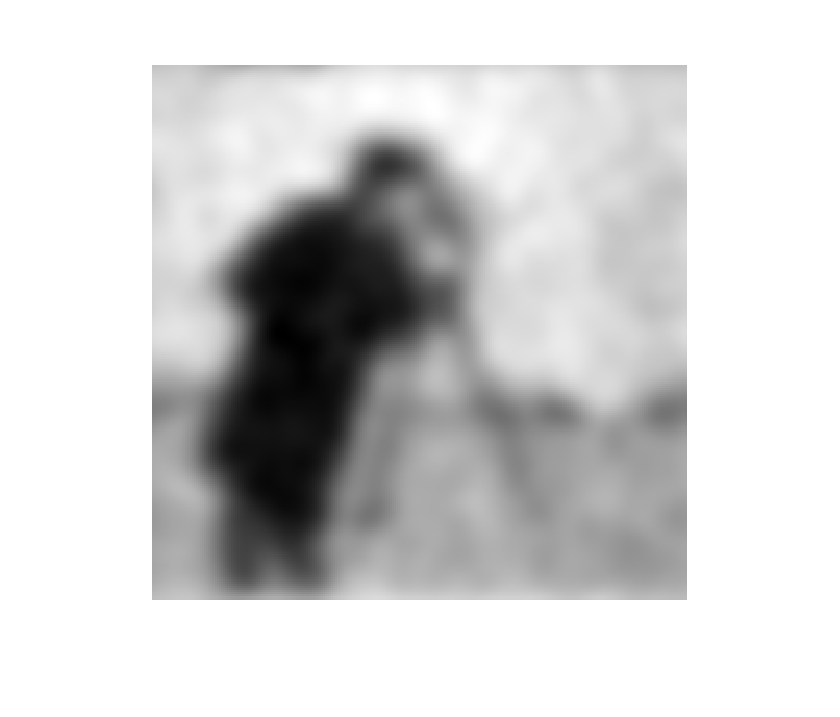
\includegraphics[scale=0.42]{Figures/UPRE_Solution_DFT_2D.eps}
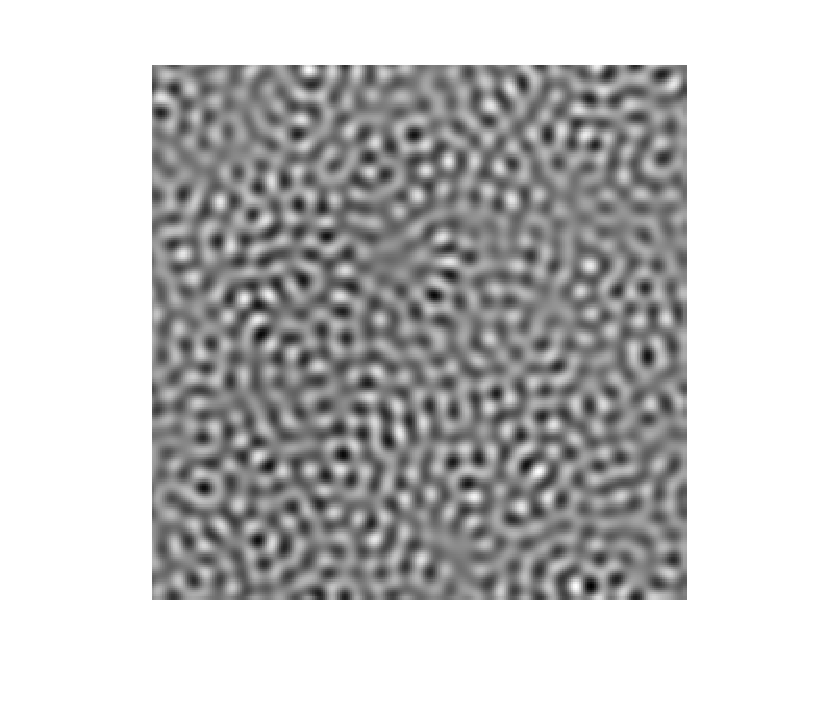
\includegraphics[scale=0.42]{Figures/UPRE_SolutionFail_DFT_2D.eps}
\caption{(Left) An example of a two-dimensional regularized solution, where the regularization parameter was selected using the UPRE method on a $65 \times 65$ downsampling of the original problem. (Right) A regularized solution for a parameter selected from a $33 \times 33$ downsampling.}
\end{figure}
\end{frame}

\section{Conclusions and future work}

\begin{frame}
\frametitle{Conclusions and future work}
\underline{Conclusions}:
\begin{itemize}
\item The numerical results demonstrate some potential viability of downsampling to obtain regularization parameters
\item The test examples do not reflect the appropriate methodology needed for practical examples
\item Main contribution of the current work has been to provide DCT and DFT derivations of the UPRE, GCV, and discrepancy principle functions, as well as related statistics
\end{itemize}
\underline{Future work}:
\begin{itemize}
\item Quantify the statistics of the regularization parameters when downsampling is applied \\
\item Investigate situations where multiple data sets are available \cite{ChungEspanol2017} \\
\item Move to three-dimensional problems such as computed tomography and subsurface imaging by gravitational measurements \cite{ABT}
\end{itemize}
\end{frame}

%\begin{frame}[allowframebreaks]
%\frametitle{References}
%
%\end{frame}

\bibliographystyle{siam}
\bibliography{Parameter-Estimation}

\end{document}